\documentclass[11pt,letterpaper,final]{report}
\usepackage[utf8]{inputenc}
\usepackage[francais]{babel}
\usepackage[T1]{fontenc}
\usepackage{amsmath}
\usepackage{amsfonts}
\usepackage{amssymb}
\usepackage{graphicx}
\usepackage{lmodern}
\usepackage[left=2.54cm,right=2.54cm,top=2.54cm,bottom=2.54cm]{geometry}
\begin{document}
\chapter{Cross validation entre les différentes plateformes de simulations}
Dans ce chapitre, les simulateurs seront comparés selon les paramètres des simulations critiques (courant dans les électroaimants, tension aux bornes des électroaimants, courant d'entrée, tension du bus CC, etc.). Les différences seront analysées selon les sous-modèles implantés, qui seront détaillés plus loin dans cet ouvrage. Les sous-modèles se séparent en plusieurs catégories, soit les simulations représentant l'AFE, celles représentant le convertisseur CC-CC et celles représentant un montage avec un AFE et un convertisseur CC-CC. Il est à noté que les temps de simulation qui seront employés pour fins d'analyse sont de 50$\mu$s, de 5$\mu$s et de 1$\mu s$. 

\section{Différences entre PSIM et SPS}
Cette section va décrire quelques différences au sein de nos 
simulations. Les IGBT de SPS sont modélisés comme idéaux tandis que ceux de PSIM ne le sont pas, sur Psim il y a des pertes par commutation faibles mais non négligeable. De plus, les IGBT de SPS intègre un snubber RC contre lequel la simulation ne fonctionne pas si on met des valeurs nuls. Pour compenser sur PSIM, nous avons mis en parallèle de chaque IGBT une charge RC de  50k$\Omega$. Ne voulant utiliser qu'une résistance, sur SPS nous avons mis les condensateurs à l'infini tandis que sur PSIM elles sont à zéro.
\section{Pont DCP/DCN: Validation PSIM/SPS}
\subsection{Hacheur 4 quadrants}
Le hacheur 4 quadrants, à proprement parlé, est constitué de 4 interrupteurs IGBT commandés au moyen d'une régulation MLI. La figure~\ref{hach} présente une représentation schématique d'un tel convertisseur. Ce type de montage est un montage de base utilisé afin de valider le concept de fonctionnement d'un convertisseur CC-CC et afin d'établir la méthodologie de comparaison des simulations.

\begin{figure}[htb]
\centering
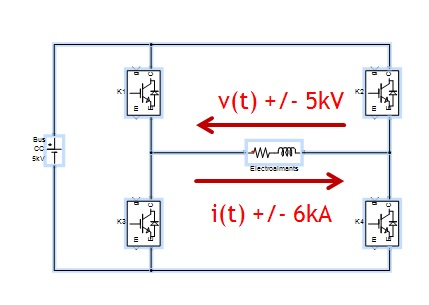
\includegraphics[scale=1]{Fig/Hacheur4Quadrants/Hacheur.jpg}
\caption{Pont en H a 4 intérrupteurs}.
\label{hach}
\end{figure}

\subsubsection{Vérification pour un pas de calcul de 50$\mu$s}
Cette section présente les courbes d'intérêt pour un pas de calcul discret de 50$\mu$s. La figure \ref{comp_PSIM_SPS} présente le courant à la charge sur PSIM et SPS pour un pas de calcul de 50 $\mu$s. Sur cette figure, on remarque que les différences entre les deux courants avoisinent les 25A. Aussi, la courbe de PSIM est décalée d'environ 150$\mu$s vers la droite par rapport à celle de SPS. On remarque que les résultats des simulations sont décalés jusqu'à 100A de la valeur de référence voulu. 

\begin{figure}[htb]
\centering
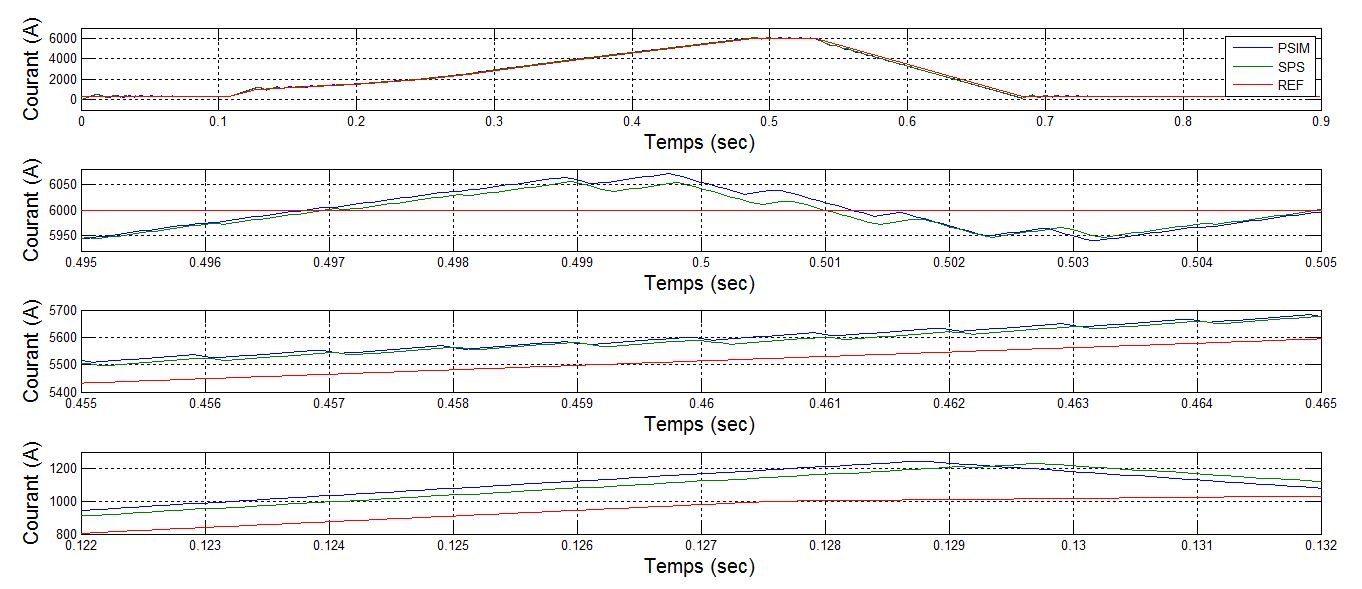
\includegraphics[scale=0.5]{Fig/Hacheur4Quadrants/HacheurCourantCharge50u.jpg}
\caption{Courant à la charge sur PSIM et SPS pour un pas de calcul de 50$\mu$s}.
\label{comp_PSIM_SPS}
\end{figure}
Sur la figure~\ref{err_cou} qui présente la tension à la charge, nous observons que les deux simulations donne les mêmes résultats à part le fait que le résultat de SPS est décalé d'environs 100$\mu$s vers la droite de celle de PSIM.

\begin{figure}[htb]
\centering
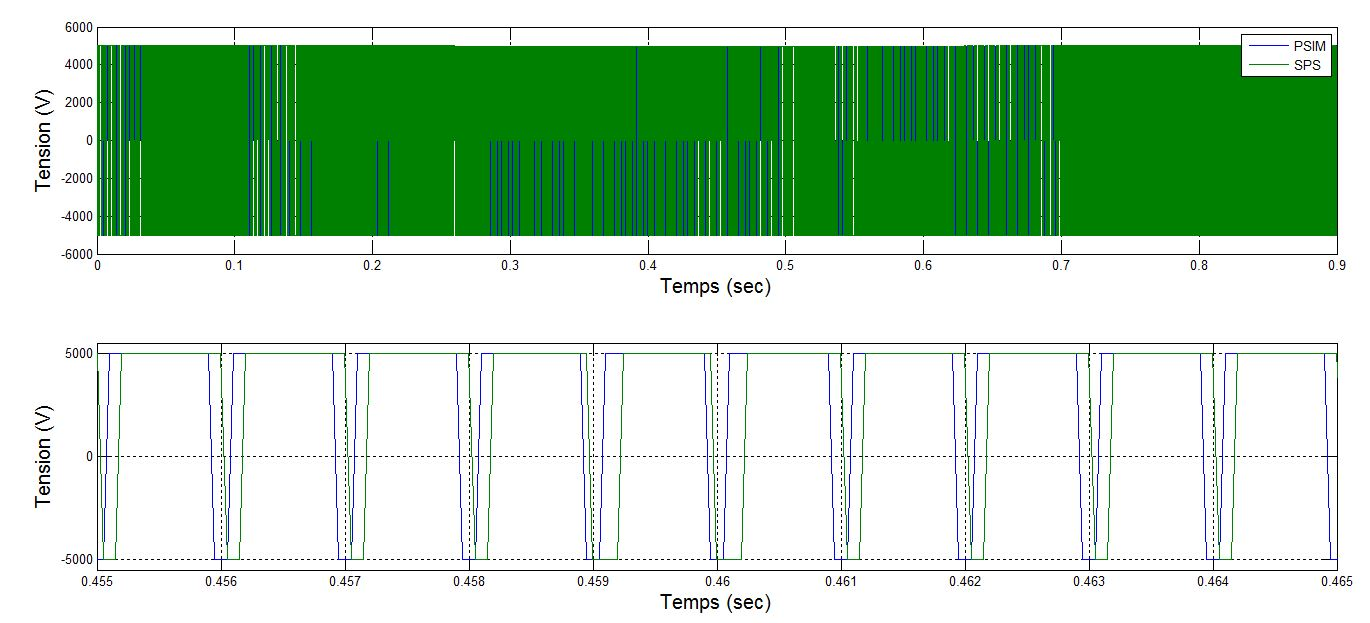
\includegraphics[scale=0.5]{Fig/Hacheur4Quadrants/HacheurTensionCharge50u.jpg}
\caption{Tension aux bornes de la charge sur PSIM et SPS pour un pas de calcul de 50$\mu$s}
\label{err_cou}
\end{figure}

La figure~\ref{hc_IG_ten_50} représente la tension aux bornes d'un IGBT pour le hacheur 4 quadrants. On remarque que les résultats sont pas toutes identiques mais la fréquence est la même. La différence observé est dû à l'algorithme de résolution de chacune des simulations. Sur SPS la simulation est discrétisé et a un passage par zéro l'algorithme change d'euler a une méthode trapézoïdale. Tandis que sur PSIM la simulation est résolu en continu.
\begin{figure}[htb]
\centering
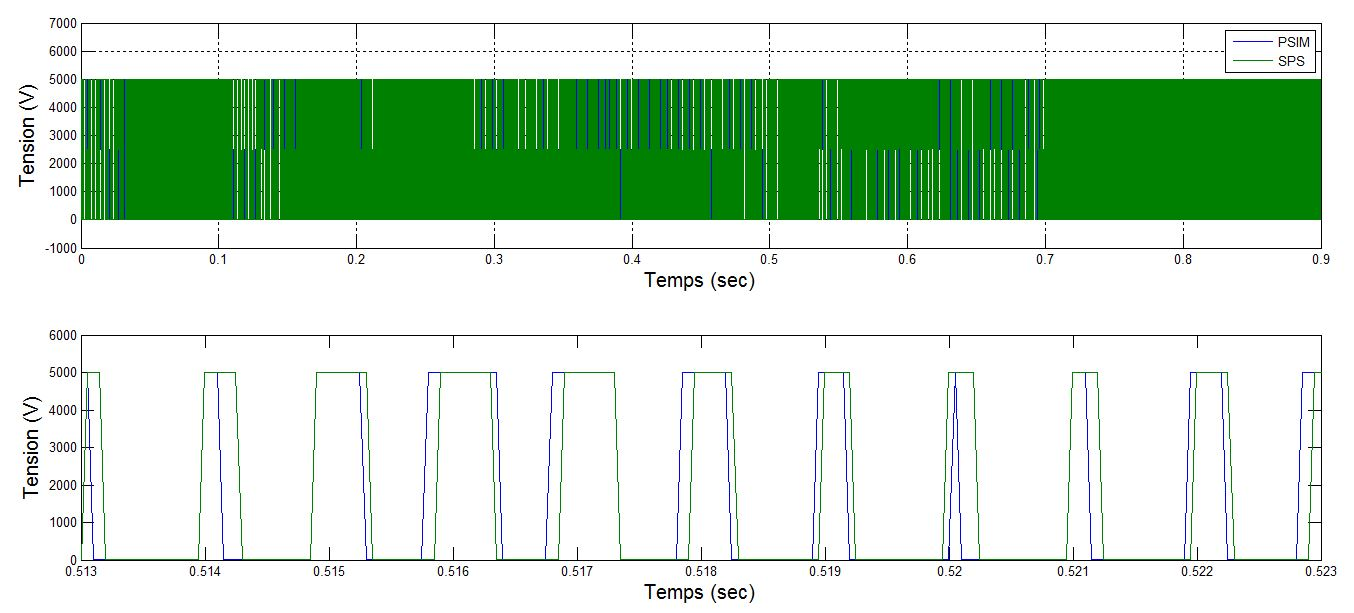
\includegraphics[scale=0.5]{Fig/Hacheur4Quadrants/HacheurTensionIGBT50u.jpg}
\caption{Tension aux bornes d'un IGBT sur PSIM et SPS pour un pas de calcul de 50$\mu$s}
\label{hc_IG_ten_50}
\end{figure}

\clearpage
\subsubsection{Vérification pour un pas de calcul de 5$\mu$s}
Cette section présente les courbes d'intérêt pour un pas de calcul discret de 5$\mu$s. À ce pas de calcul le résultat est beaucoup plus précis. La figure~\ref{hc_cou_ch_5}
montre le courant à charge pour un pas de 5$\mu$s.  Le courant à la charge observé en différentes période entre PSIM et SPS est en phase. On remarque par contre que l'oscillation de courant de SPS est décalé d'environs 10A, mais qu'elles suivent très bien la référence de courant voulu avec une différence d'environs 18A.
\begin{figure}[htb]
\centering
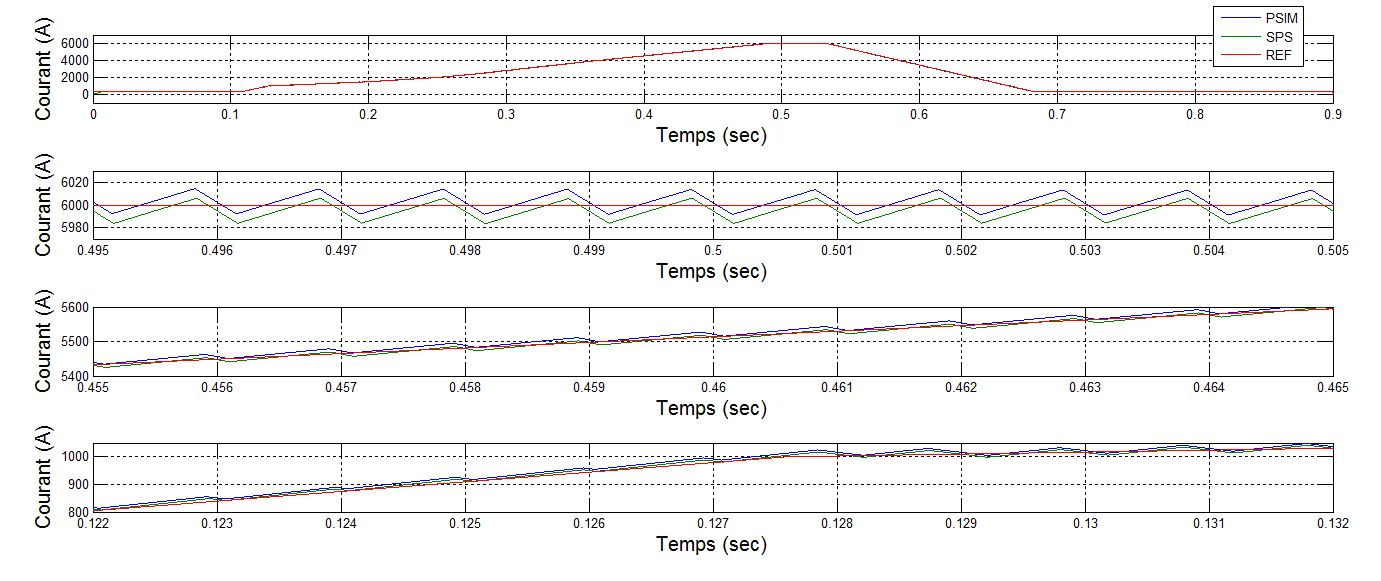
\includegraphics[scale=0.5]{Fig/Hacheur4Quadrants/HacheurCourantCharge5u.jpg}
\caption{Courant traversant la charge sur PSIM et SPS pour un pas de calcul de 5$\mu$s}
\label{hc_cou_ch_5}
\end{figure}
Les deux figures suivantes~\ref{hc_ten_ch_5} et ~\ref{hc_IG_ten_5} qui représente la tension à la charge et aux bornes de l'IGBT ont des courbes entre PSIM et SPS qui se superpose très bien, qui donne pratiquement le même résultat.


\begin{figure}[htb]
\centering
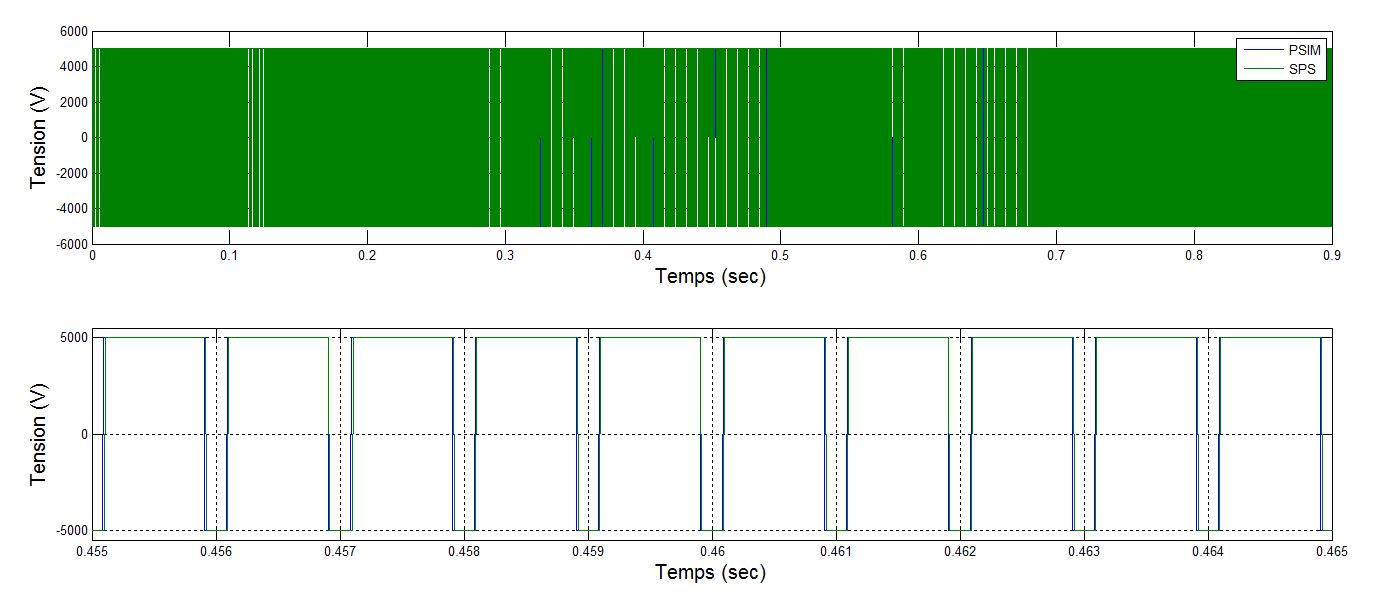
\includegraphics[scale=0.5]{Fig/Hacheur4Quadrants/HacheurTensionCharge5u.jpg}
\caption{Tension aux bornes de la charge sur PSIM et SPS pour un pas de calcul de 5$\mu$s}
\label{hc_ten_ch_5}
\end{figure}


\begin{figure}[htb]
\centering
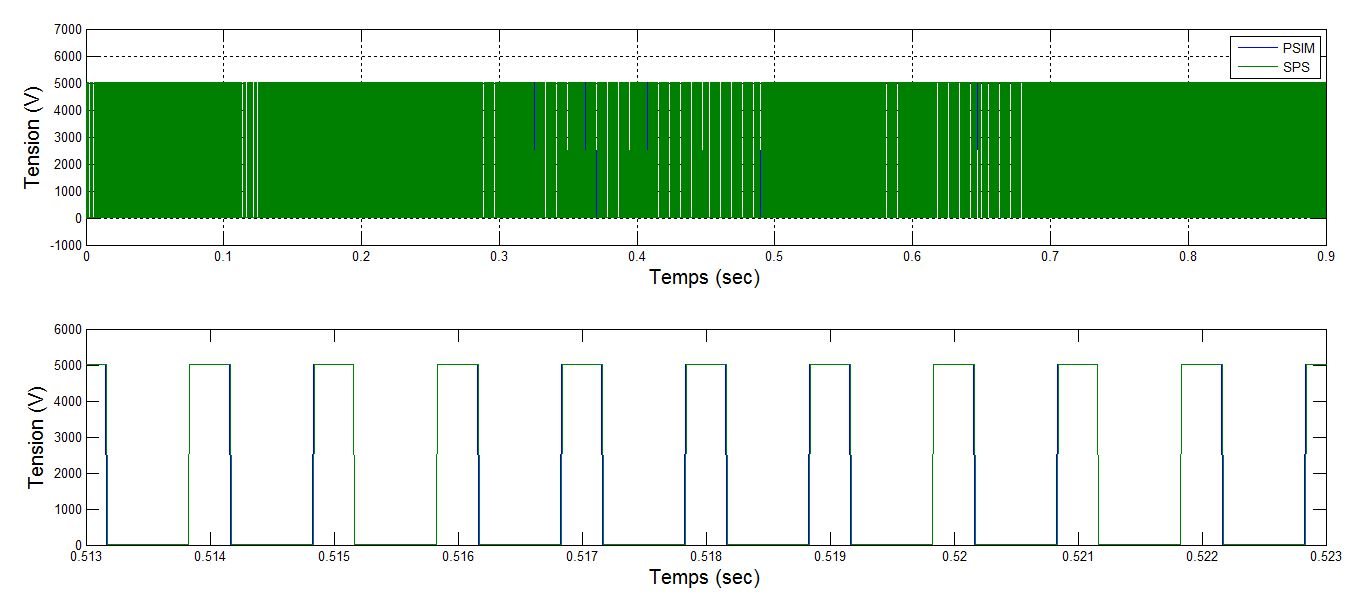
\includegraphics[scale=0.5]{Fig/Hacheur4Quadrants/HacheurTensionIGBT5u.jpg}
\caption{Tension aux bornes d'un IGBT sur PSIM et SPS pour un pas de calcul de 5$\mu$s}
\label{hc_IG_ten_5}
\end{figure}

\clearpage
\subsubsection{Vérification pour un pas de calcul de 1$\mu$s}
Cette section présente les courbes d'intérêt pour un pas de calcul discret de 1$\mu$s. On remarque que les résultats des figures~\ref{hc_cou_ch_1}, ~\ref{hc_ten_ch_1}, ~\ref{hc_IG_cou_1} et ~\ref{hc_IG_ten_1} qui représentent le courant à la charge, la tension à la charge, le courant et tension au niveau de IGBT à un pas de calcul de 1$\mu$s, donne les mêmes résultats qui ceux obtenu pour un pas de 5$\mu$s. 


\begin{figure}[htb]
\centering
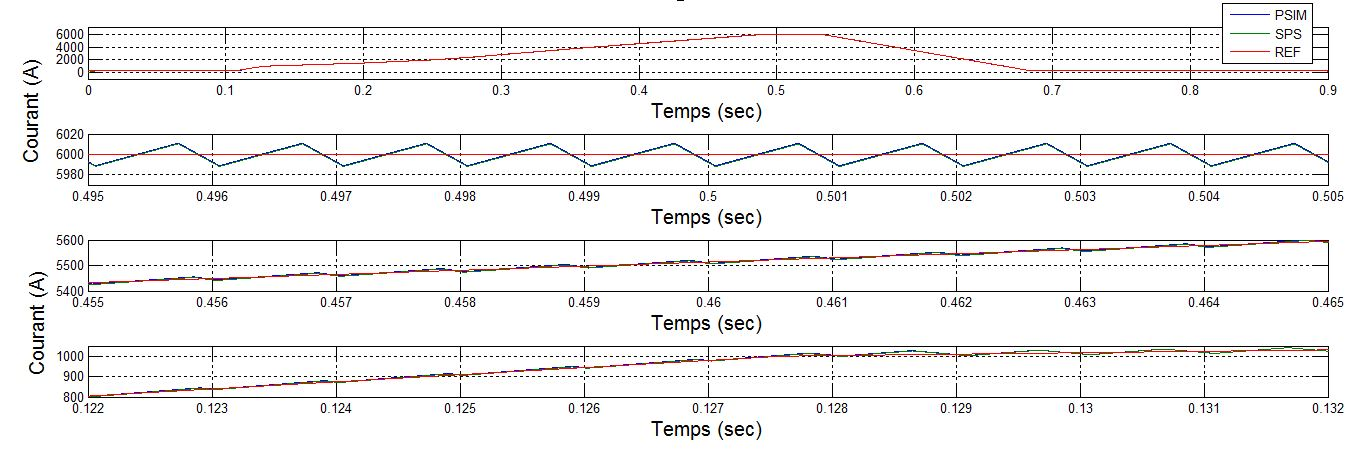
\includegraphics[scale=0.5]{Fig/Hacheur4Quadrants/HacheurCourantCharge1u.jpg}
\caption{Courant traversant la charge sur PSIM et SPS pour un pas de calcul de 1$\mu$s}
\label{hc_cou_ch_1}
\end{figure}


\begin{figure}[htb]
\centering
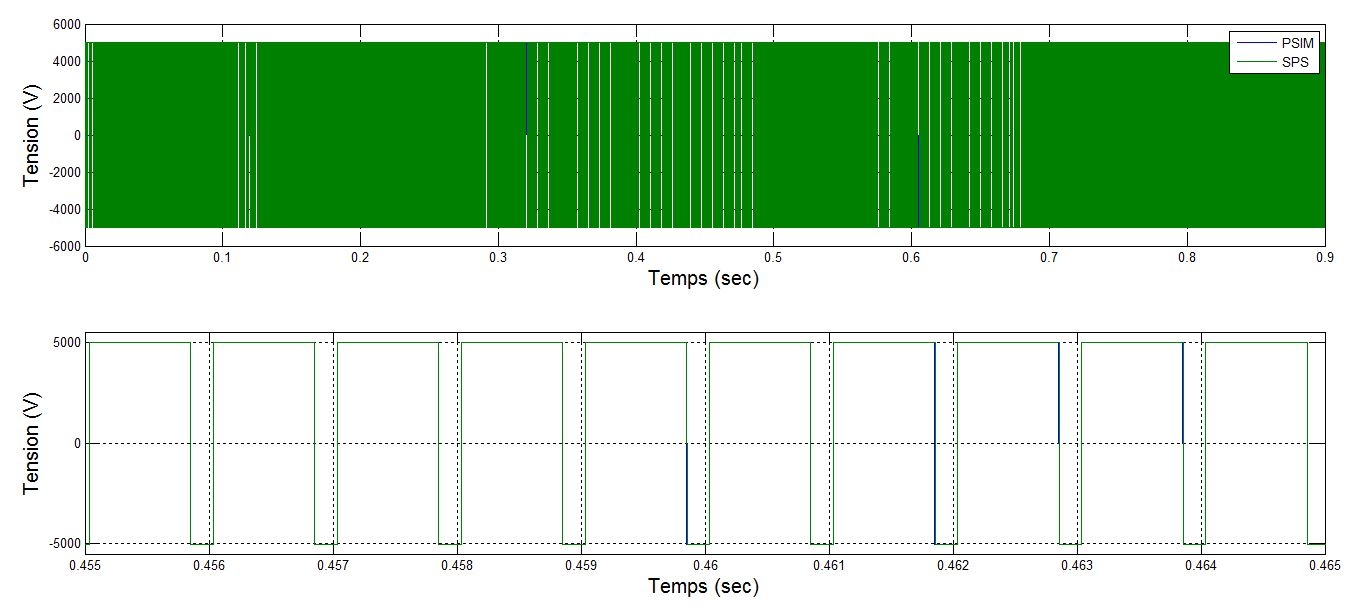
\includegraphics[scale=0.5]{Fig/Hacheur4Quadrants/HacheurTensionCharge1u.jpg}
\caption{Tension aux bornes de la charge sur PSIM et SPS pour un pas de calcul de 1$\mu$s}
\label{hc_ten_ch_1}
\end{figure}


\begin{figure}[htb]
\centering
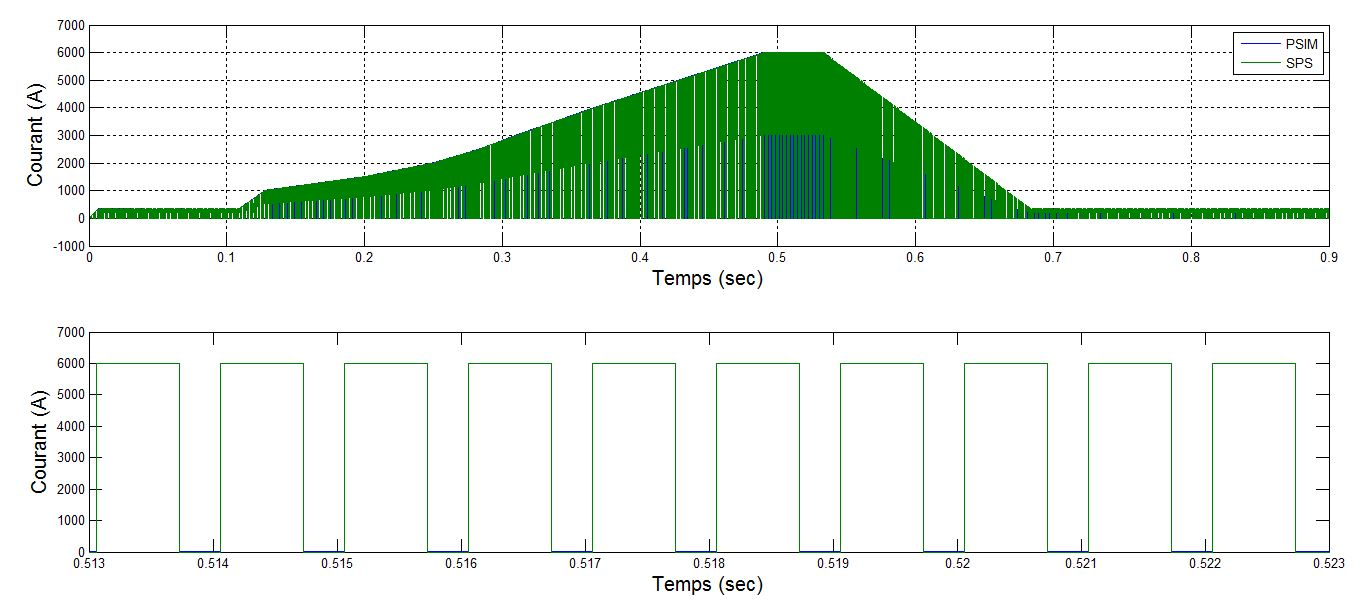
\includegraphics[scale=0.5]{Fig/Hacheur4Quadrants/HacheurCourantIGBT1u.jpg}
\caption{Courant traversant un IGBT sur PSIM et SPS pour un pas de calcul de 1$\mu$s}
\label{hc_IG_cou_1}
\end{figure}

\begin{figure}[htb]
\centering
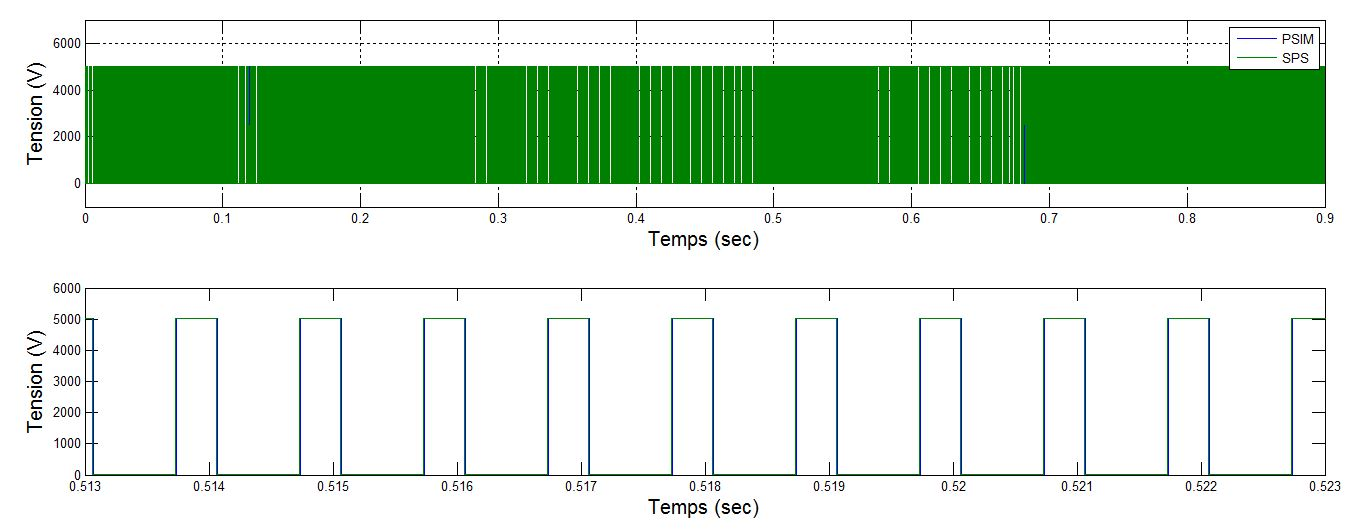
\includegraphics[scale=0.5]{Fig/Hacheur4Quadrants/HacheurTensionIGBT1u.jpg}
\caption{Tension aux bornes d'un IGBT sur PSIM et SPS pour un pas de calcul de 1$\mu$s}
\label{hc_IG_ten_1}
\end{figure}


\clearpage

\subsection{DCP/DCN}
Le DCP/DCN est un convertisseur CC-CC, qui représente un système plus complexe du fonctionnement du hacheur 4 quadrants. Il est composé de 24 interrupteurs IGBT/DIODE commandé avec une commande MLI ainsi que de 12 diodes de retour.
\subsubsection{Vérification à un pas de calcul de 50$\mu$s}
Cette section présente les courbes d'intérêt pour un pas de calcul discret de 50$\mu$s. La figure~\ref{DC_ch_cou_50} qui représente la courant à la charge à un pas de calcul de 50$\mu$s montre que le résultat de PSIM et SPS ne vont pas à la même fréquence, la fréquence de SPS est plus élevé que celle de PSIM. Par contre, ils sont décalés d'environs 18A par rapport au courant de référence. On remarque que les résultats obtenus ne comporte pas de dépassement.

Les figures~\ref{DC_ch_ten_50},~\ref{DC_IG_cou_50} et ~\ref{DC_IG_ten_50}


\begin{figure}[htb]
\centering
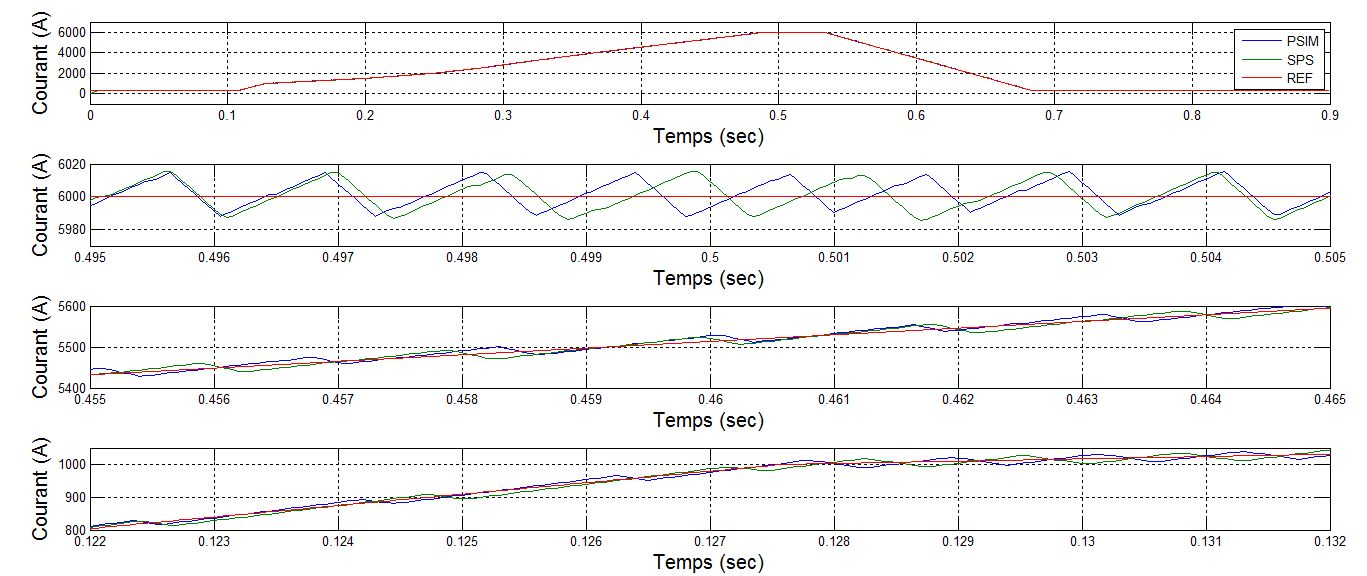
\includegraphics[scale=0.5]{Fig/DCPDCN/DCPCourantCharge50u.jpg}
\caption{Courant traversant la charge sur PSIM et SPS pour un pas de calcul de 50$\mu$s}
\label{DC_ch_cou_50}
\end{figure}


\begin{figure}[htb]
\centering
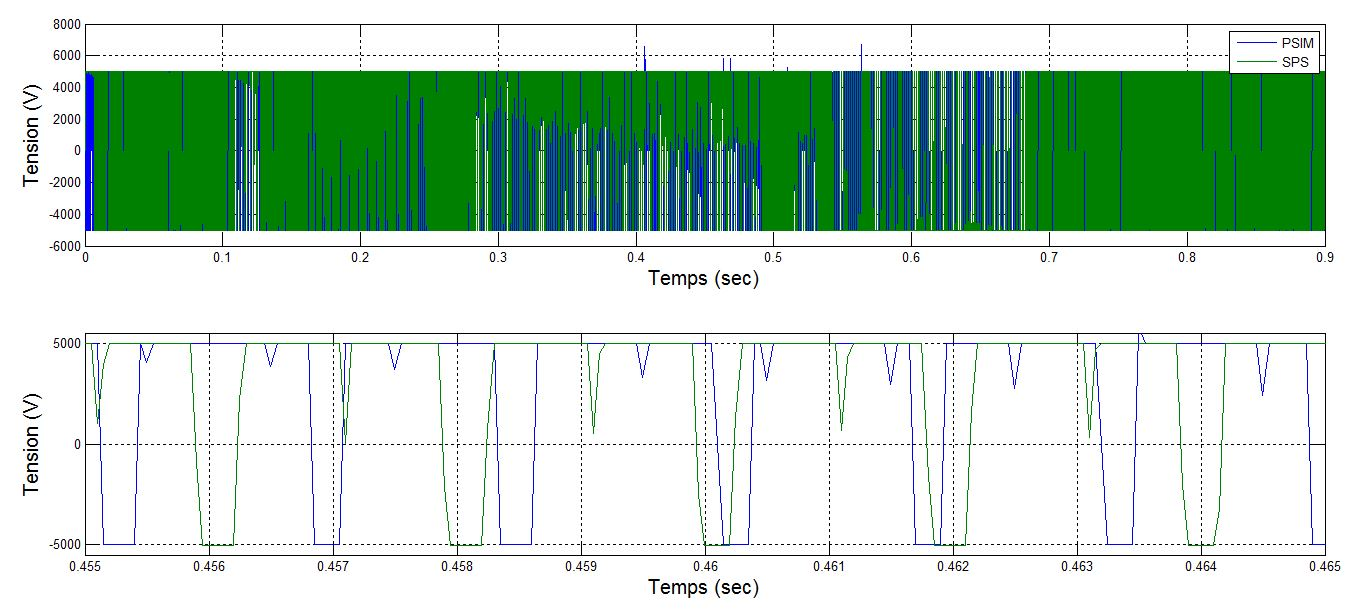
\includegraphics[scale=0.5]{Fig/DCPDCN/DCPTensionCharge50u.jpg}
\caption{Tension aux bornes de la charge sur PSIM et SPS pour un pas de calcul de 50$\mu$s}.
\label{DC_ch_ten_50}
\end{figure}

\begin{figure}[htb]
\centering
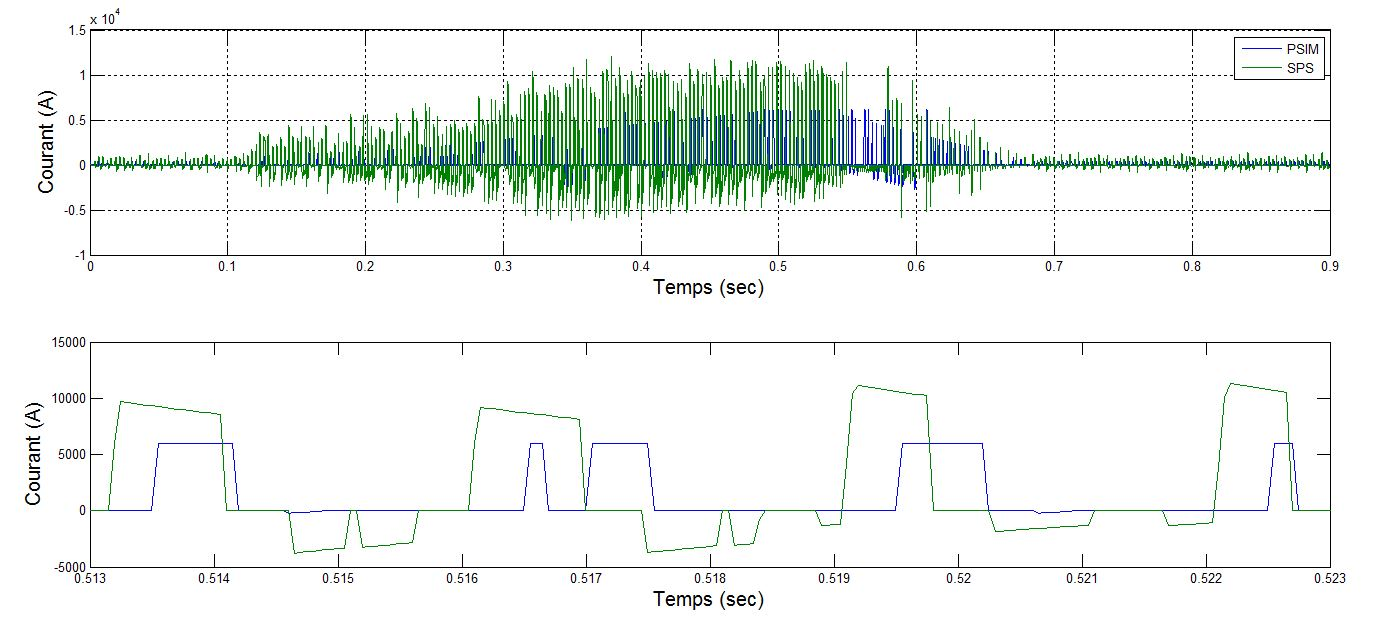
\includegraphics[scale=0.5]{Fig/DCPDCN/DCPCourantIGBT50u.jpg}
\caption{Courant traversant un IGBT sur PSIM et SPS pour un pas de calcul de 50$\mu$s}
\label{DC_IG_cou_50}
\end{figure}

\begin{figure}[htb]
\centering
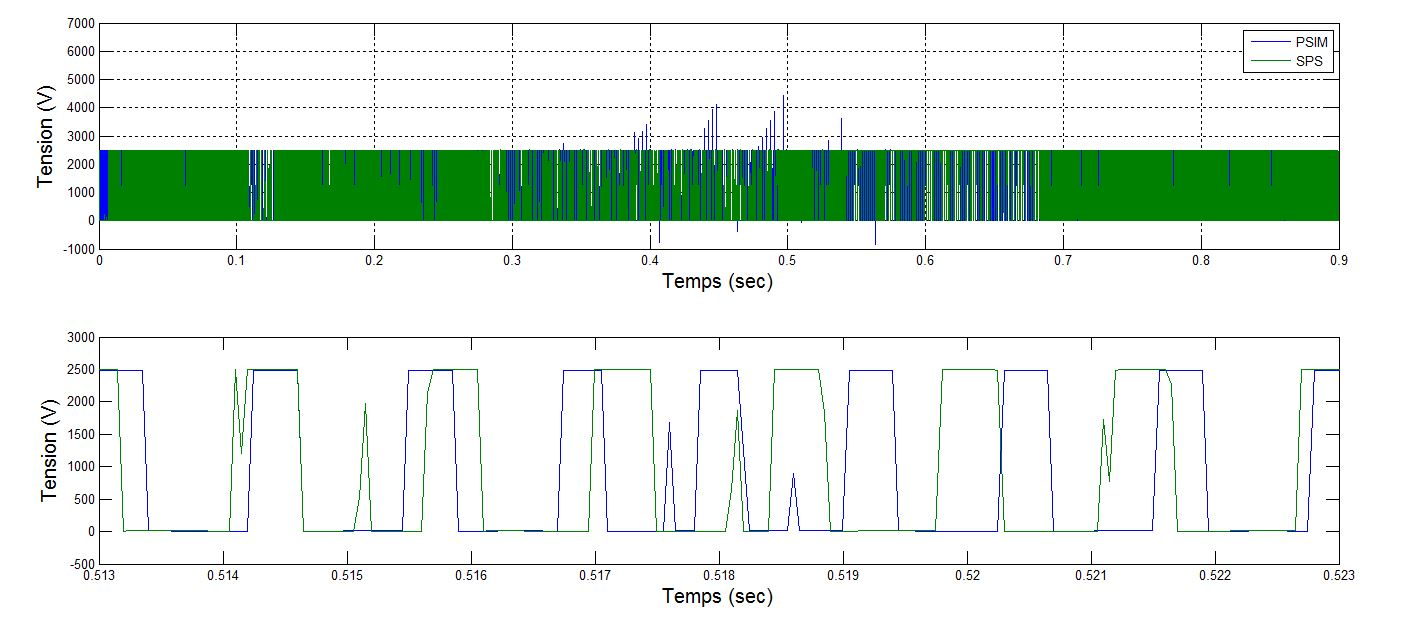
\includegraphics[scale=0.5]{Fig/DCPDCN/DCPTensionIGBT50u.jpg}
\caption{Tension au niveau d'un IGBT sur PSIM et SPS pour un pas de calcul de 50$\mu$s}
\label{DC_IG_ten_50}
\end{figure}


\clearpage

\subsubsection{Vérification à pas de calcul de 5$\mu$s}
Cette section présente les courbes d'intérêt pour un pas de calcul discret de 5$\mu$s.

\begin{figure}[htb]
\centering
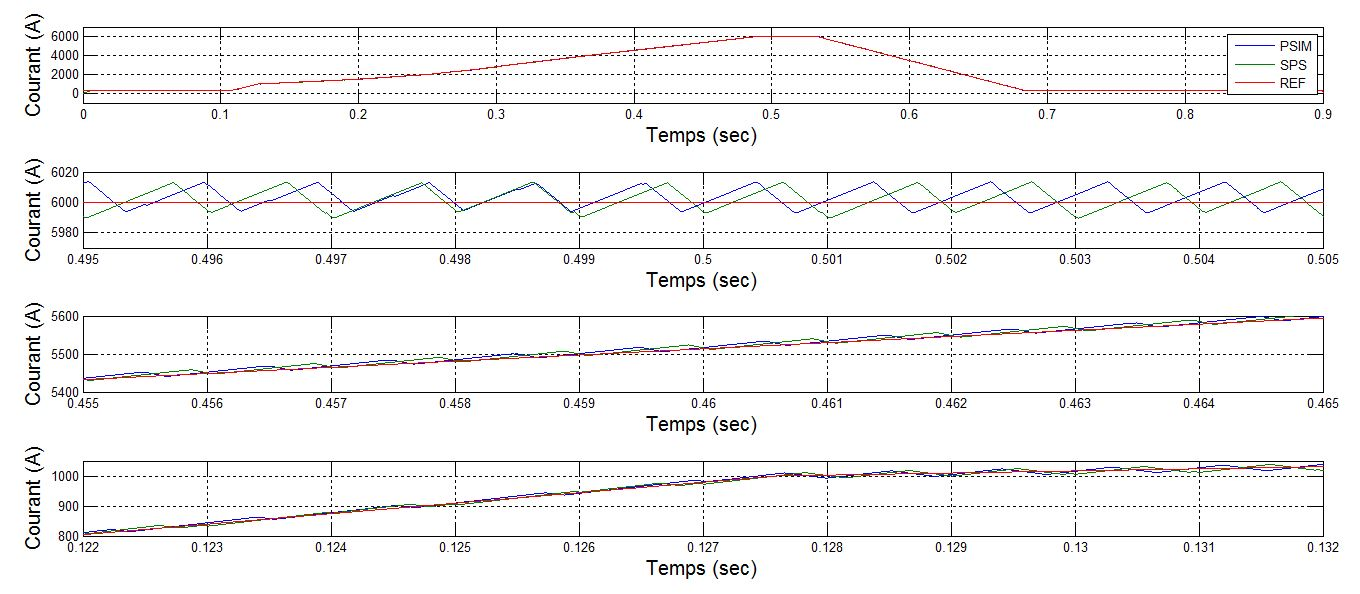
\includegraphics[scale=0.5]{Fig/DCPDCN/DCPCourantCharge5u.jpg}
\caption{Courant traversant la charge sur PSIM et SPS pour un pas de calcul de 5$\mu$s}
\label{DC_ch_cou_5}
\end{figure}


\begin{figure}[htb]
\centering
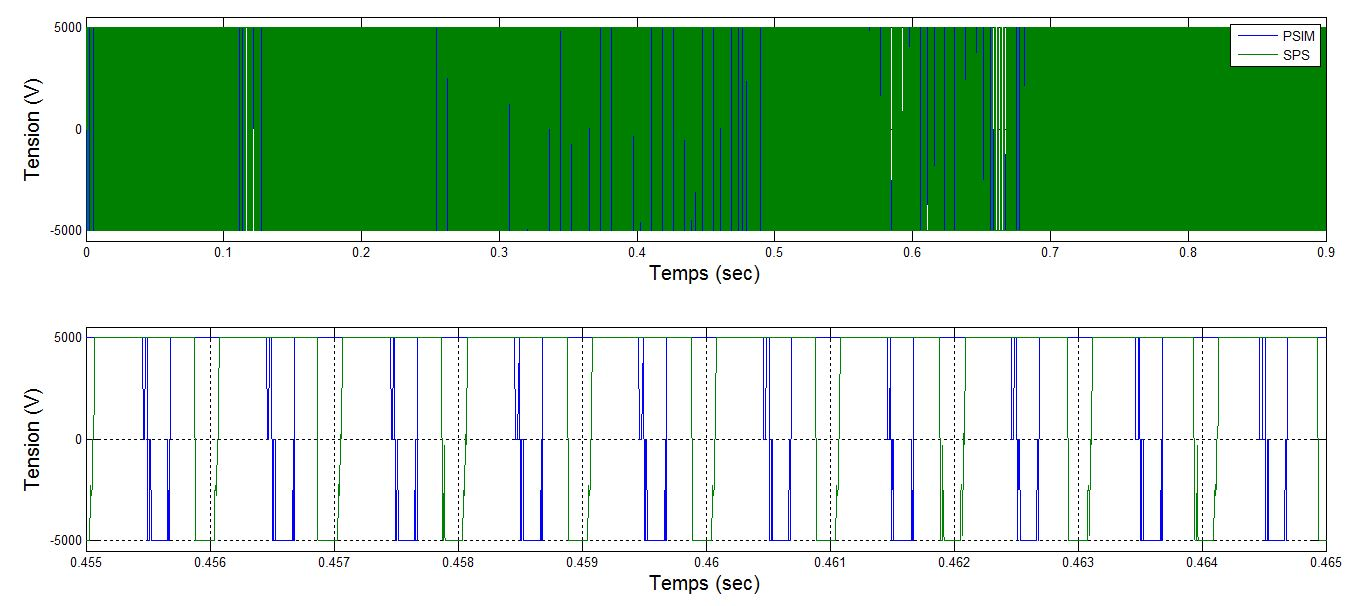
\includegraphics[scale=0.5]{Fig/DCPDCN/DCPTensionCharge5u.jpg}
\caption{Tension aux bornes de la charge sur PSIM et SPS pour un pas de calcul de 5$\mu$s}
\label{DC_ch_ten_5}
\end{figure}

\begin{figure}[htb]
\centering
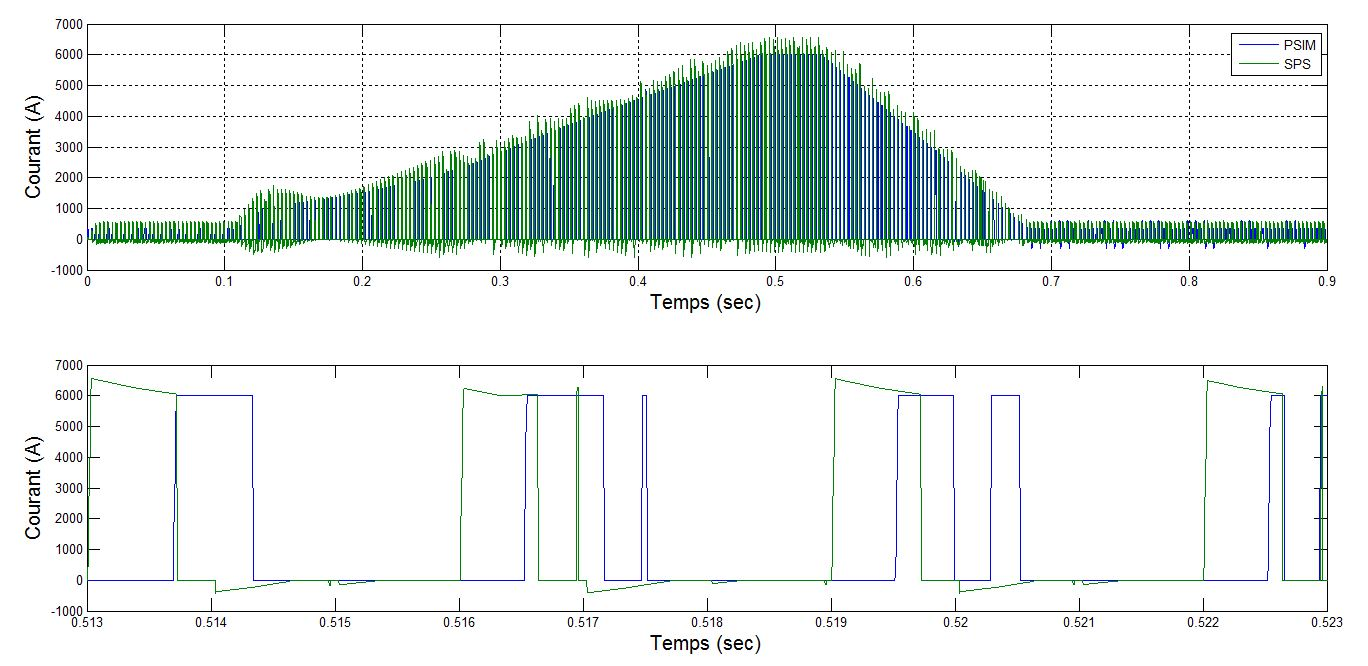
\includegraphics[scale=0.5]{Fig/DCPDCN/DCPCourantIGBT5u.jpg}
\caption{Courant traversant un IGBT sur PSIM et SPS pour un pas de calcul de 5$\mu$s}
\label{DC_IG_cou_5}
\end{figure}



\begin{figure}[htb]
\centering
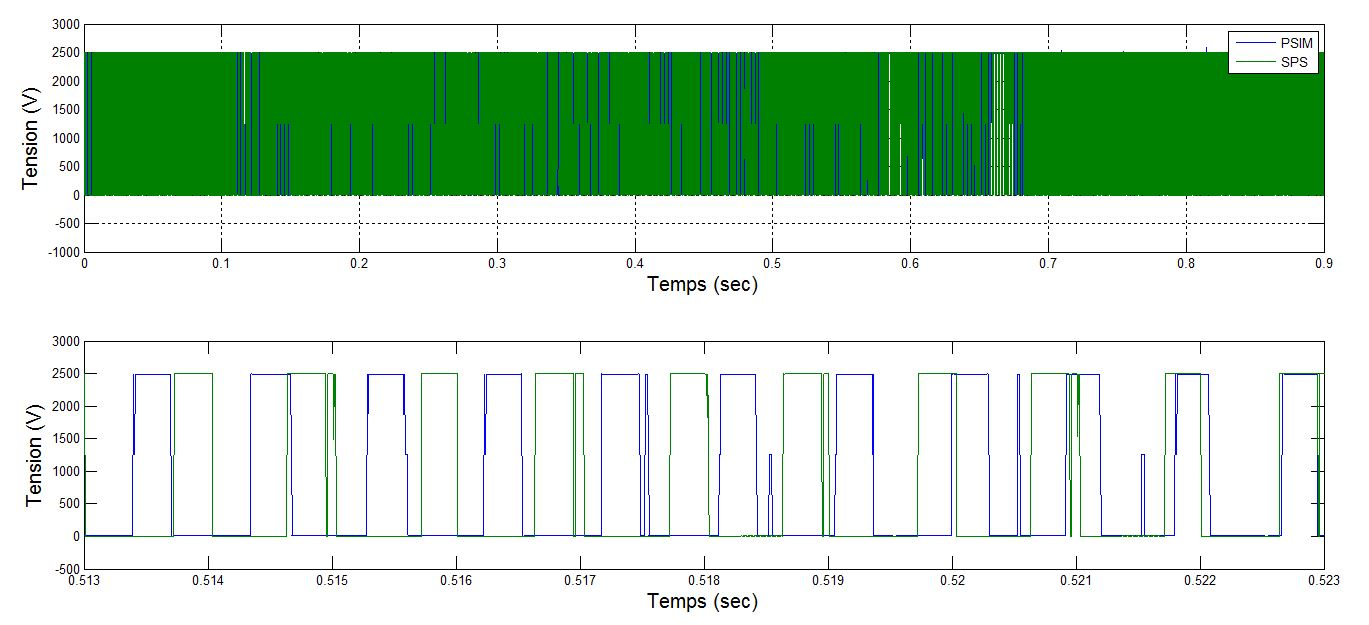
\includegraphics[scale=0.5]{Fig/DCPDCN/DCPTensionIGBT5u.jpg}
\caption{Tension traversant un IGBT sur PSIM et SPS pour un pas de calcul de 5$\mu$s}
\label{DC_IG_ten_5}
\end{figure}



\clearpage
\subsubsection{Vérification à un pas de calcul de 1us}
Cette section présente les courbes d'intérêt pour un pas de calcul discret de 1$\mu$s.


\begin{figure}[htb]
\centering
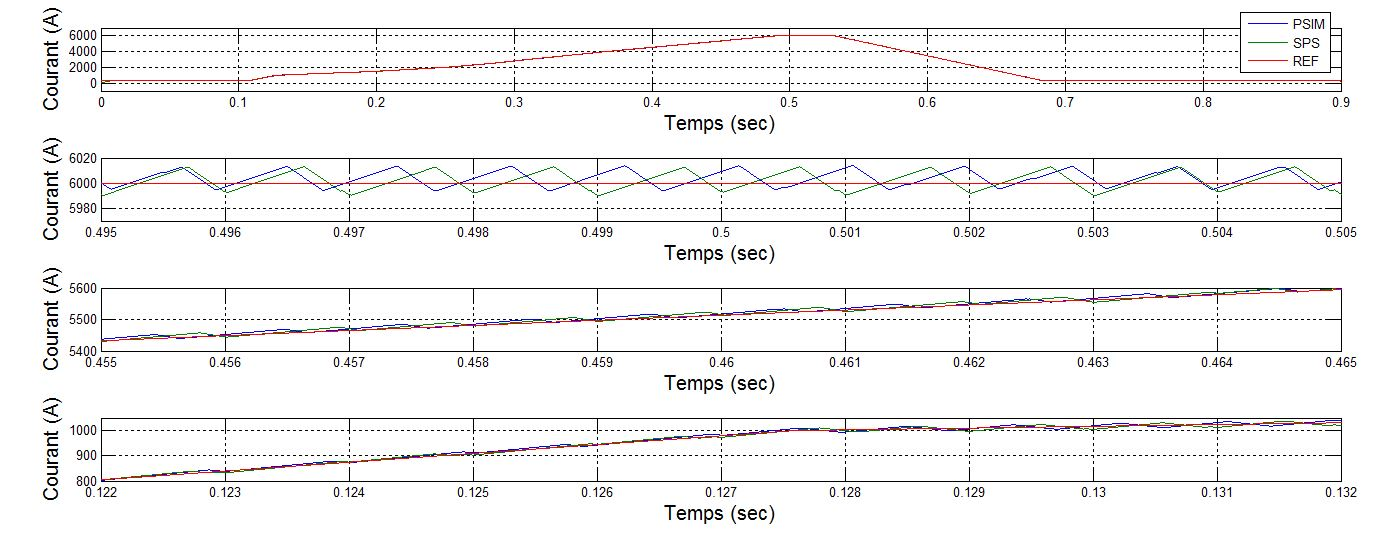
\includegraphics[scale=0.5]{Fig/DCPDCN/DCPCourantCharge1u.jpg}
\caption{Courant traversant la charge sur PSIM et SPS pour un pas de calcul de 1$\mu$s}
\label{DC_ch_cou_1}
\end{figure}


\begin{figure}[htb]
\centering
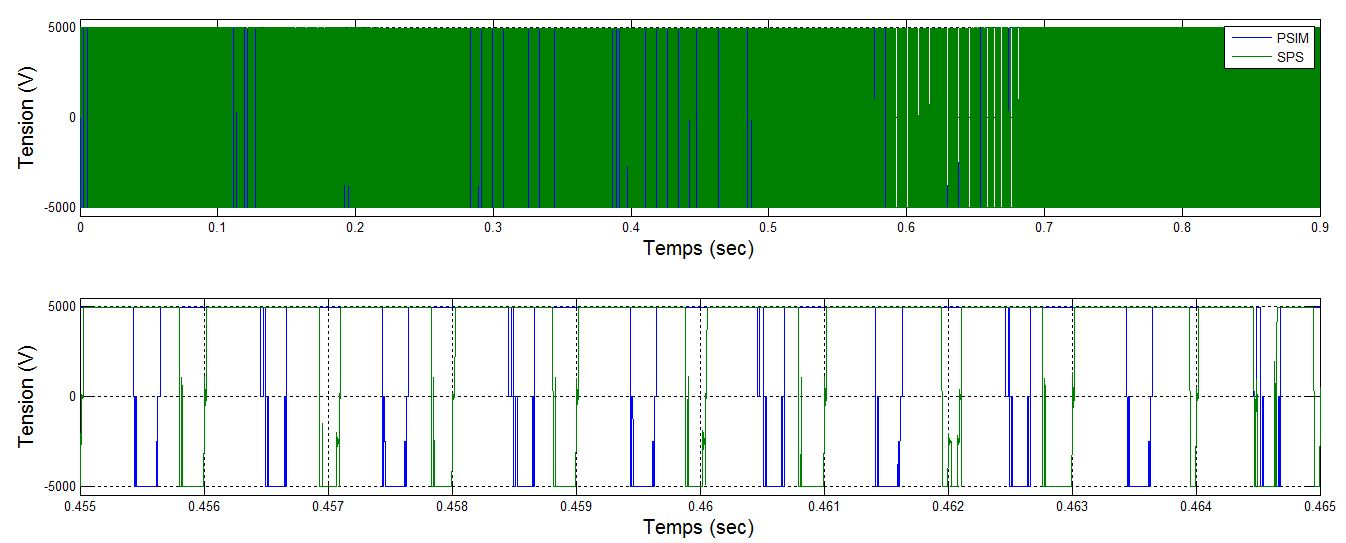
\includegraphics[scale=0.5]{Fig/DCPDCN/DCPTensionCharge1u.jpg}
\caption{Tension aux bornes de la charge sur PSIM et SPS pour un pas de calcul de 1$\mu$s}
\label{DC_ch_ten_1}
\end{figure}


\begin{figure}[htb]
\centering
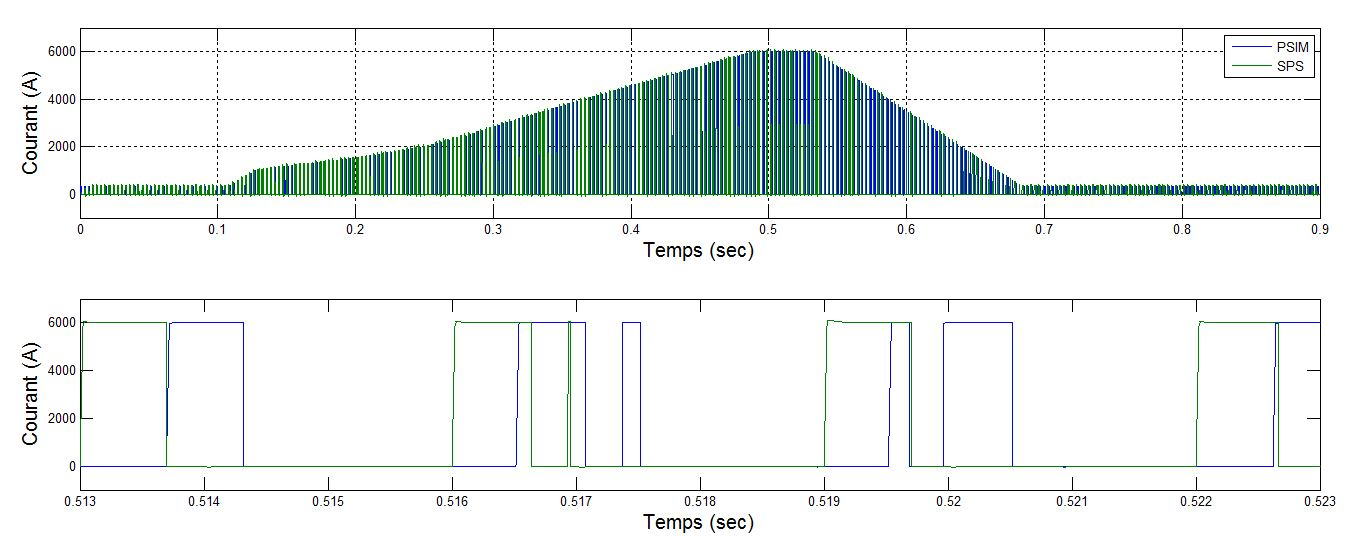
\includegraphics[scale=0.5]{Fig/DCPDCN/DCPCourantIGBT1u.jpg}
\caption{Courant traversant un IGBT sur PSIM et SPS pour un pas de calcul de 1$\mu$s}
\label{DC_IG_cou_1}
\end{figure}


\begin{figure}[htb]
\centering
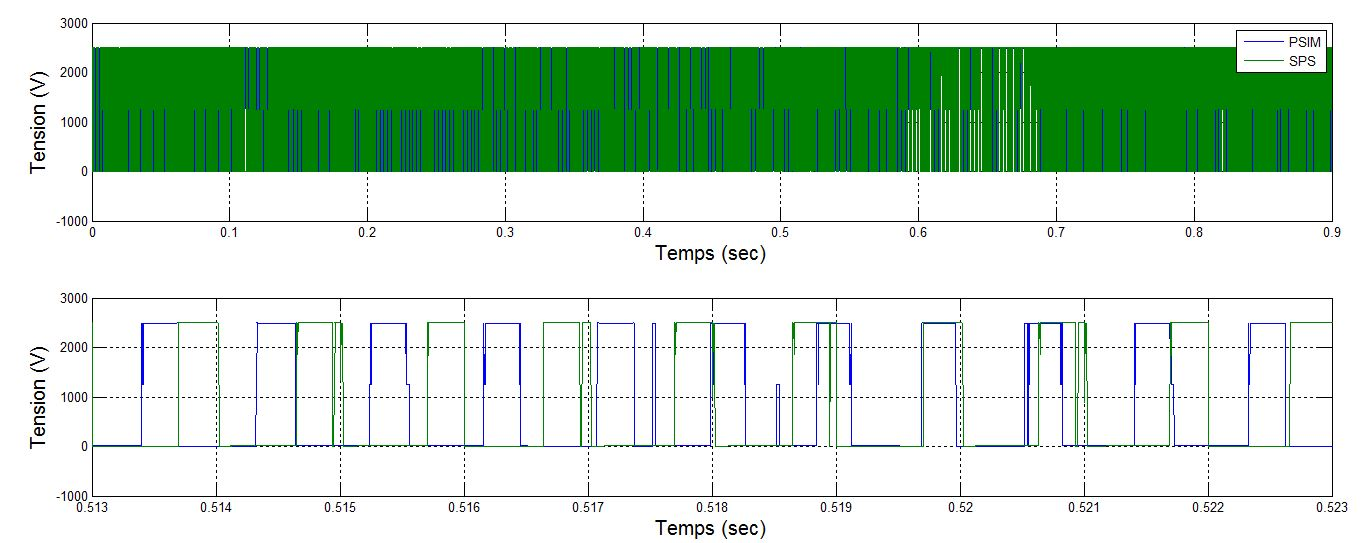
\includegraphics[scale=0.5]{Fig/DCPDCN/DCPTensionIGBT1u.jpg}
\caption{Tension aux bornes d'un IGBT sur PSIM et SPS pour un pas de calcul de 1$\mu$s}
\label{DC_IG_ten_1}
\end{figure}

\clearpage
\section{AFE: Validation PSIM/SPS}
\subsection{AFE source idéal}
\subsubsection{Vérification pour un pas de calcul de 1$\mu$s}

\begin{figure}[htb]
\centering
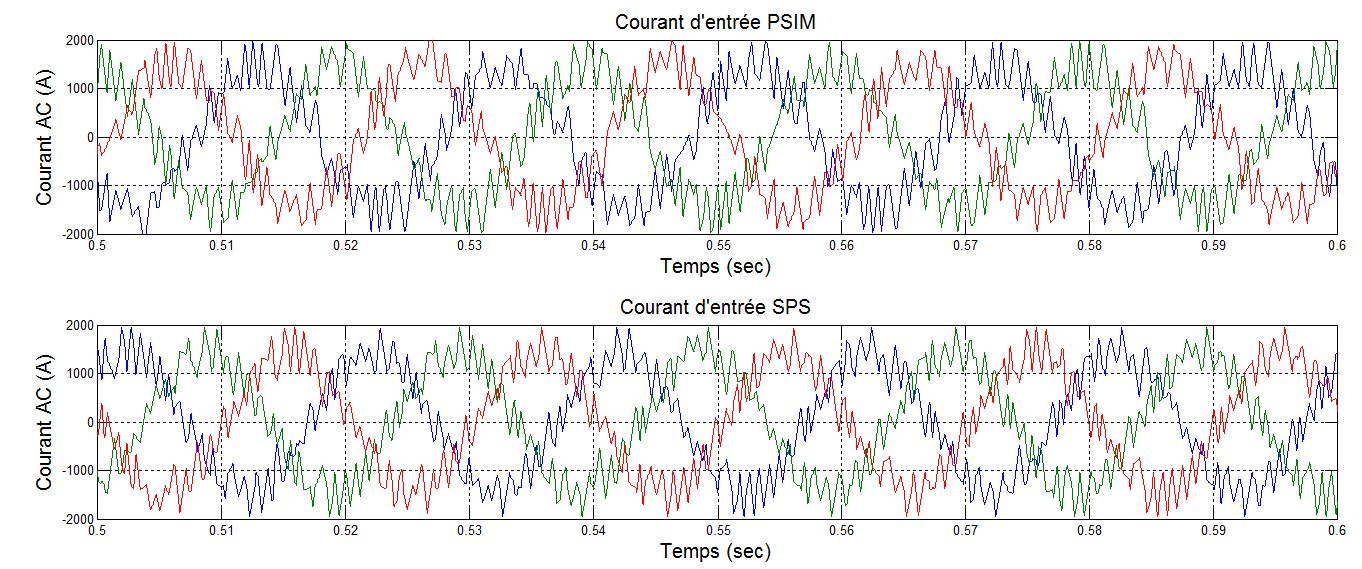
\includegraphics[scale=0.5]{Fig/AFEIDEAL/CourantAC.jpg}
\caption{Le courant d'entrée à 1$\mu$s}
\label{AF_I_cou}
\end{figure}

\begin{figure}[htb]
\centering
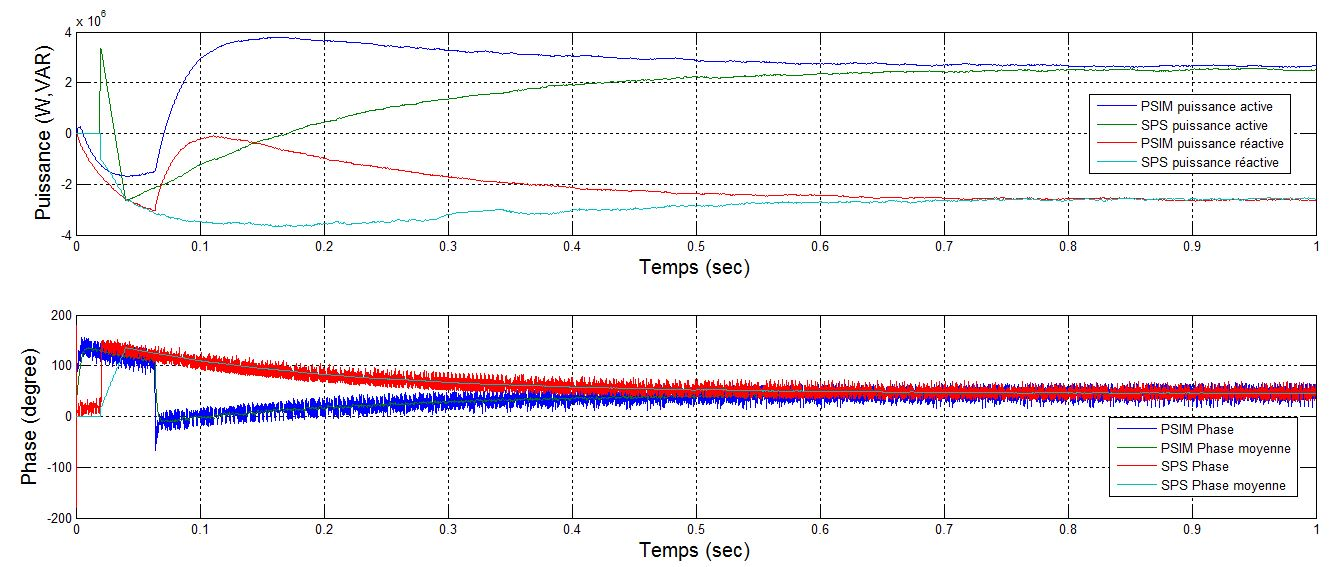
\includegraphics[scale=0.5]{Fig/AFEIDEAL/pui45.jpg}
\caption{La puissance à une phase de 45 degré à 1$\mu$s}
\label{AF_I_pui_45}
\end{figure}

\begin{figure}[htb]
\centering
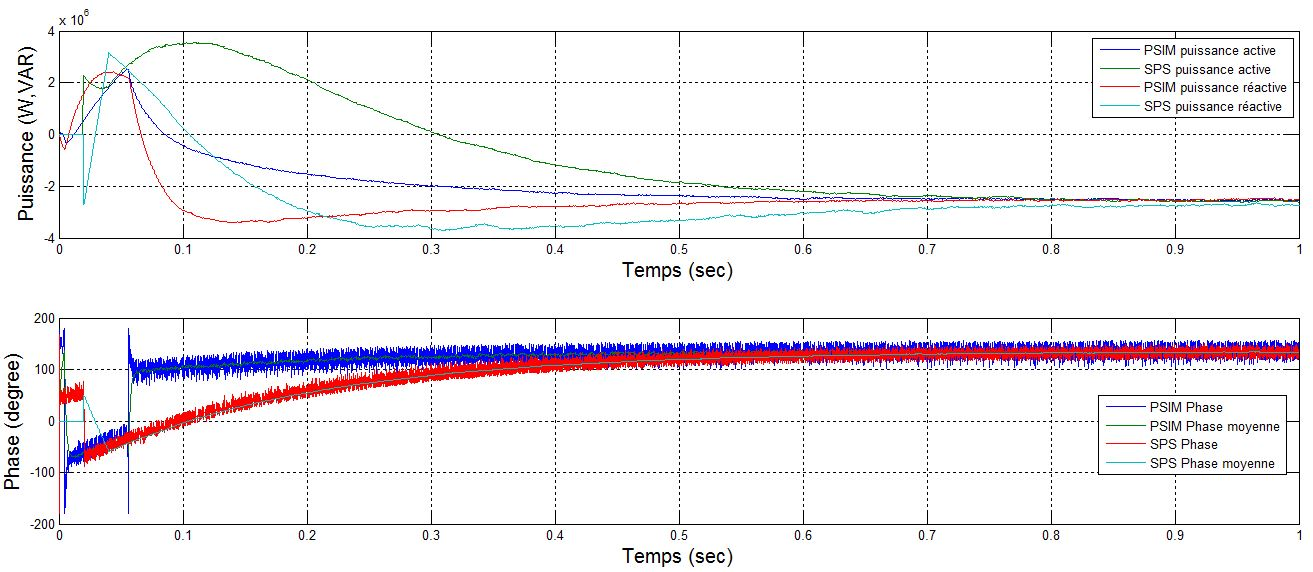
\includegraphics[scale=0.5]{Fig/AFEIDEAL/pui135.jpg}
\caption{La puissance à une phase de 135 degré à 1$\mu$s}
\label{AF_I_pui_135}
\end{figure}

\begin{figure}[htb]
\centering
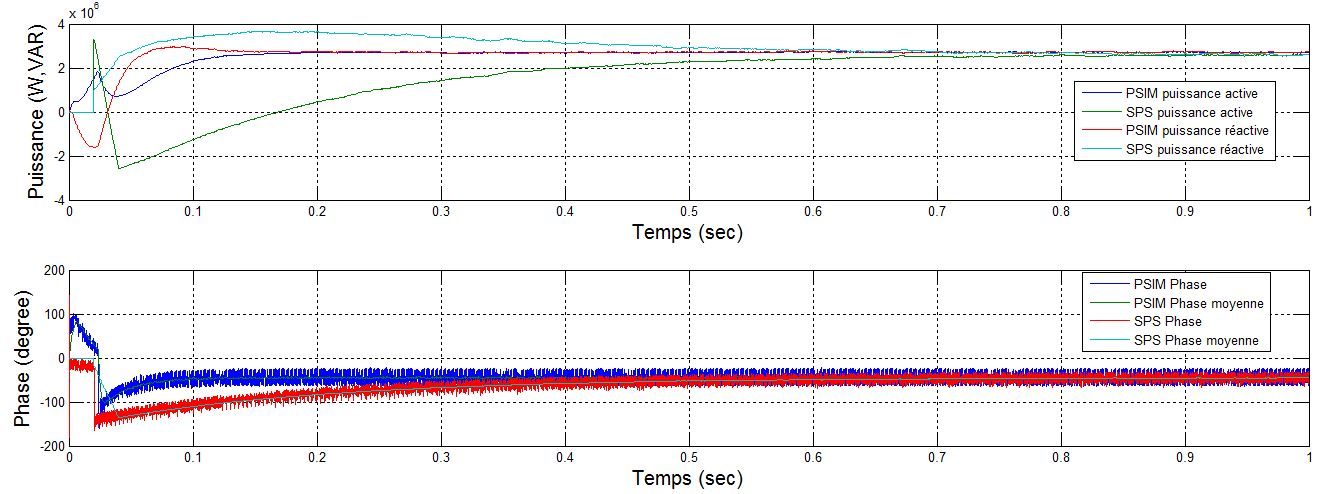
\includegraphics[scale=0.5]{Fig/AFEIDEAL/pui_45.jpg}
\caption{La puissance à une phase de -45 degré à 1$\mu$s}
\label{AF_I_pui__45}
\end{figure}

\begin{figure}[htb]
\centering
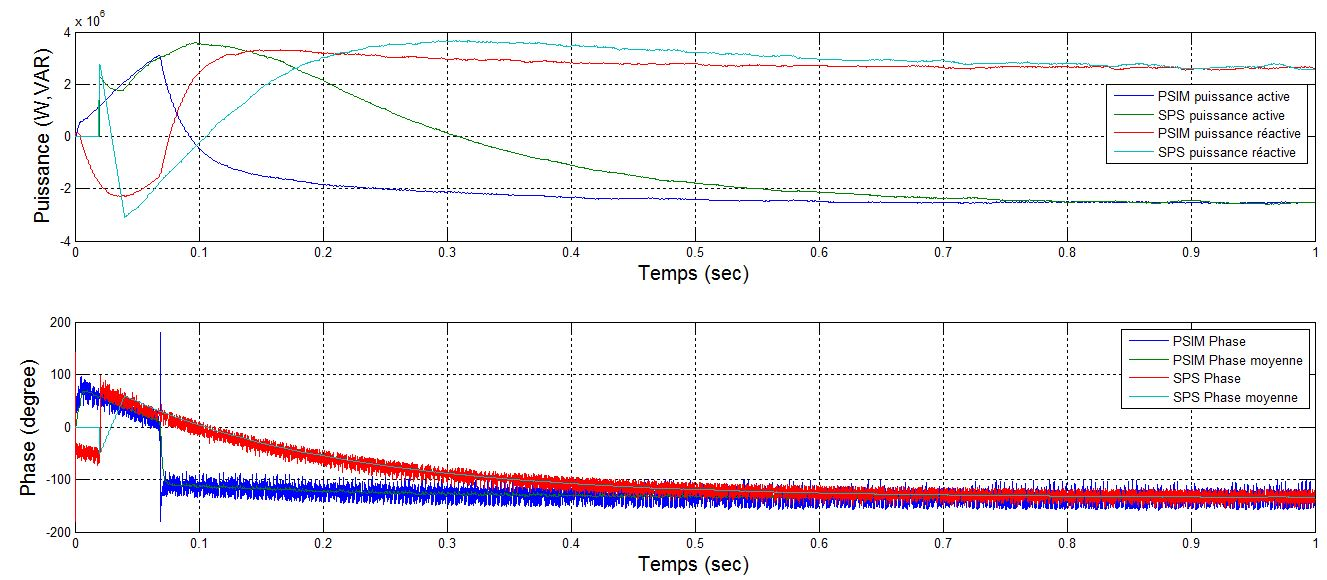
\includegraphics[scale=0.5]{Fig/AFEIDEAL/pui_135.jpg}
\caption{La puissance à une phase de -135 degré à 1$\mu$s}
\label{AF_I_pui__135}
\end{figure}

\clearpage
\subsection{AFE avec charge RC}
\subsubsection{Vérification pour un pas de calcul de 1$\mu$s}

\begin{figure}[htb]
\centering
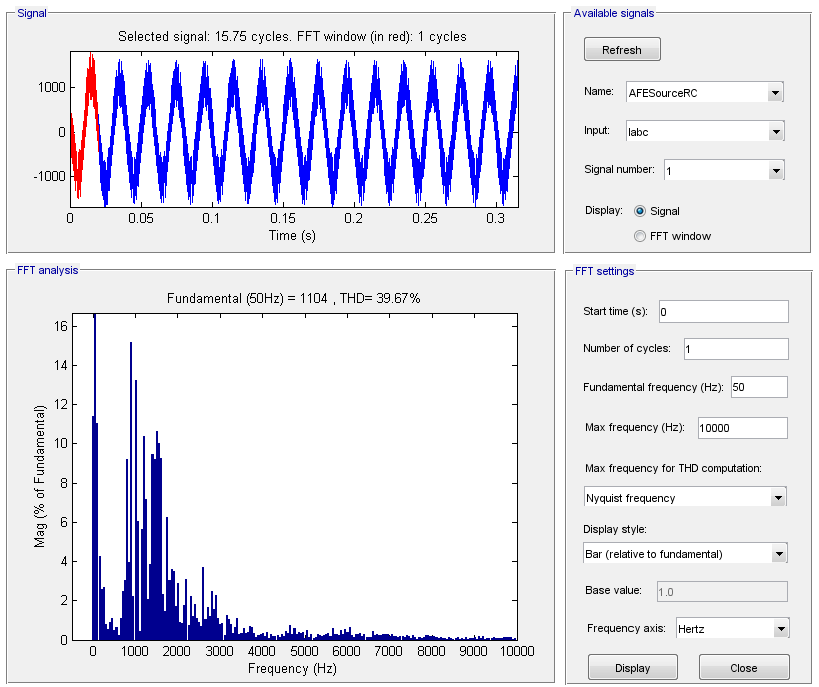
\includegraphics[scale=0.5]{Fig/AFERC/FFTAnalysisToolResult5u.png}
\caption{La FFT du courant d'entrée à 1$\mu$s}
\label{fft_RC}
\end{figure}

\begin{figure}[htb]
\centering
\includegraphics[scale=0.5]{Fig/AFERC/cour_al.jpg}
\caption{Le courant d'entrée à 1$\mu$s}
\label{AF_RC_cou}
\end{figure}

\begin{figure}[htb]
\centering
\includegraphics[scale=0.5]{Fig/AFERC/vch.jpg}
\caption{La tension à la charge à 1$\mu$s}
\label{AF_RC_ten}
\end{figure}

\begin{figure}[htb]
\centering
\includegraphics[scale=0.5]{Fig/AFERC/IGBT.jpg}
\caption{La tension et le courant au niveau d'un IGBT à 1$\mu$s}
\label{AF_RC_igbt}
\end{figure}

\clearpage
\subsection{AFE 3 level}
\subsubsection{Vérification pour un pas de calcul de 50$\mu$s}

\begin{figure}[htb]
\centering
\includegraphics[scale=0.5]{Fig/AFE3LEVEL/50u/cour_al.jpg}
\caption{Le courant d'entrée à 50$\mu$s}
\label{AF_3_cou50}
\end{figure}

\begin{figure}[htb]
\centering
\includegraphics[scale=0.5]{Fig/AFE3LEVEL/50u/vch.jpg}
\caption{La tension à la charge à 50$\mu$s}
\label{AF_3_vch50}
\end{figure}


\begin{figure}[htb]
\centering
\includegraphics[scale=0.5]{Fig/AFE3LEVEL/50u/IGBT.jpg}
\caption{La tension et le courant au niveau d'un IGBT à 50$\mu$s}
\label{AF_3_IGBT50}
\end{figure}

\begin{figure}[htb]
\centering
\includegraphics[scale=0.5]{Fig/AFE3LEVEL/50u/DIODE.jpg}
\caption{La tension et le courant au niveau d'une diode à 50$\mu$s}
\label{AF_3_DIODE50}
\end{figure}

\clearpage
\subsubsection{Vérification pour un pas de calcul de 5$\mu$s}

\begin{figure}[htb]
\centering
\includegraphics[scale=0.5]{Fig/AFE3LEVEL/5u/cour_al.jpg}
\caption{Le courant d'entrée à 5$\mu$s}
\label{AF_3_cou5}
\end{figure}

\begin{figure}[htb]
\centering
\includegraphics[scale=0.5]{Fig/AFE3LEVEL/5u/vch.jpg}
\caption{La tension à la charge à 5$\mu$s}
\label{AF_3_vch5}
\end{figure}


\begin{figure}[htb]
\centering
\includegraphics[scale=0.5]{Fig/AFE3LEVEL/5u/IGBT.jpg}
\caption{La tension et le courant au niveau d'un IGBT à 5$\mu$s}
\label{AF_3_IGBT5}
\end{figure}

\begin{figure}[htb]
\centering
\includegraphics[scale=0.5]{Fig/AFE3LEVEL/5u/DIODE.jpg}
\caption{La tension et le courant au niveau d'une diode à 5$\mu$s}
\label{AF_3_DIODE5}
\end{figure}

\clearpage
\subsubsection{Vérification pour un pas de calcul de 1$\mu$s}

\begin{figure}[htb]
\centering
\includegraphics[scale=0.5]{Fig/AFE3LEVEL/1u/cour_al.jpg}
\caption{Le courant d'entrée à 1$\mu$s}
\label{AF_3_cou}
\end{figure}

\begin{figure}[htb]
\centering
\includegraphics[scale=0.5]{Fig/AFE3LEVEL/1u/vch.jpg}
\caption{La tension à la charge à 1$\mu$s}
\label{AF_3_vch}
\end{figure}


\begin{figure}[htb]
\centering
\includegraphics[scale=0.5]{Fig/AFE3LEVEL/1u/IGBT.jpg}
\caption{La tension et le courant au niveau d'un IGBT à 1$\mu$s}
\label{AF_3_IGBT}
\end{figure}

\begin{figure}[htb]
\centering
\includegraphics[scale=0.5]{Fig/AFE3LEVEL/1u/DIODE.jpg}
\caption{La tension et le courant au niveau d'une diode à 1$\mu$s}
\label{AF_3_DIODE}
\end{figure}

\clearpage
\section{Implémentation AFE avec DCP/DCN}
\subsection{AFE 2 level avec hacheur 4 quadrants}
\subsubsection{Vérification pour un pas de calcul de 50$\mu$s}

\begin{figure}[htb]
\centering
\includegraphics[scale=0.5]{Fig/Hach_AFE/50u/cour_al.jpg}
\caption{Le courant d'entrée à 50$\mu$s}
\label{AF_HA_cou50}
\end{figure}

\begin{figure}[htb]
\centering
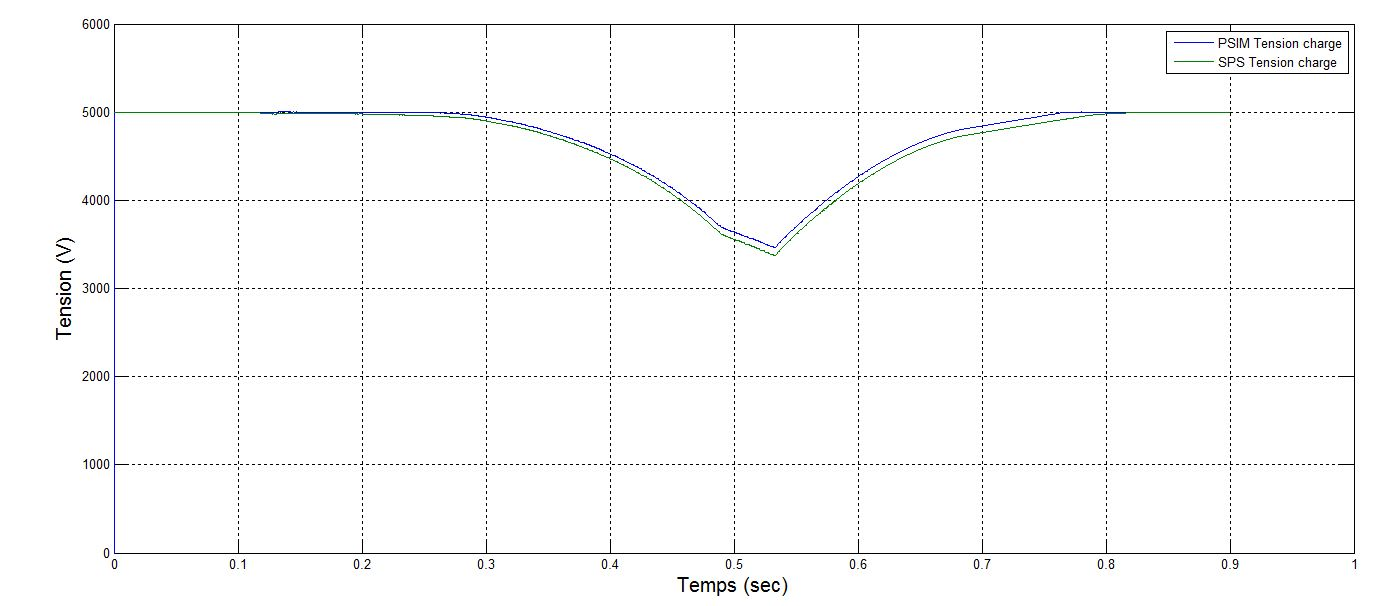
\includegraphics[scale=0.5]{Fig/Hach_AFE/50u/ten_bus.jpg}
\caption{La tension au bus à 50$\mu$s}
\label{AF_HA_vch50}
\end{figure}


\begin{figure}[htb]
\centering
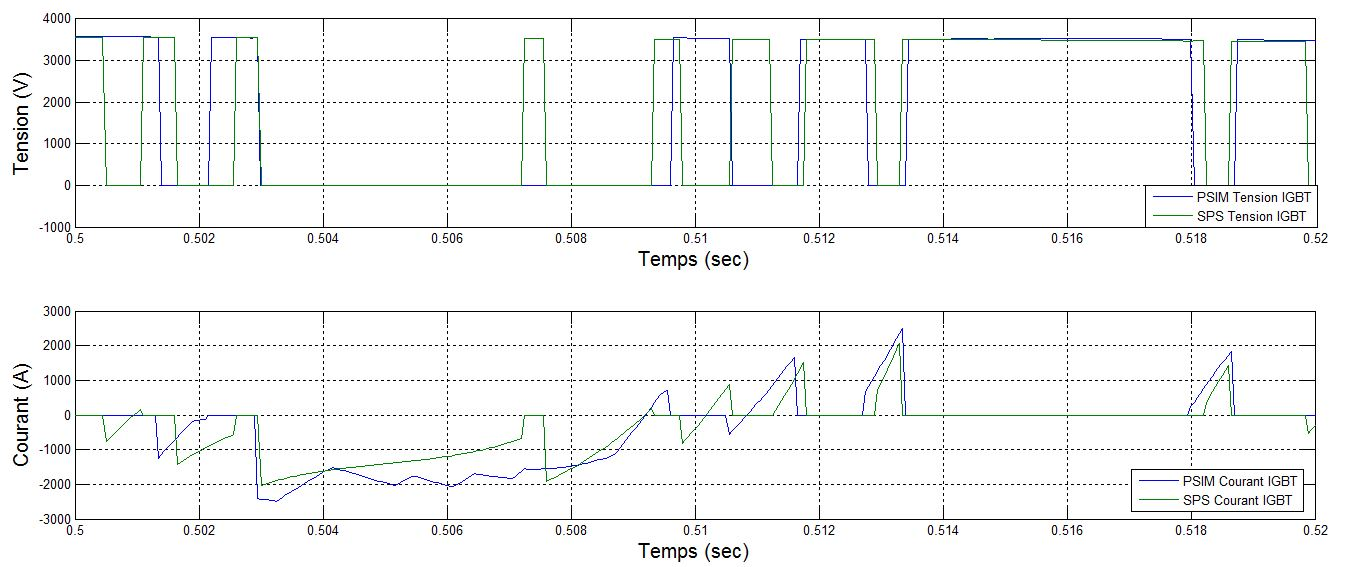
\includegraphics[scale=0.5]{Fig/Hach_AFE/50u/IGBT_AFE.jpg}
\caption{La tension et le courant au niveau d'un IGBT à 50$\mu$s au niveau de l'AFE}
\label{AF_HA_IGBT50}
\end{figure}

\begin{figure}[htb]
\centering
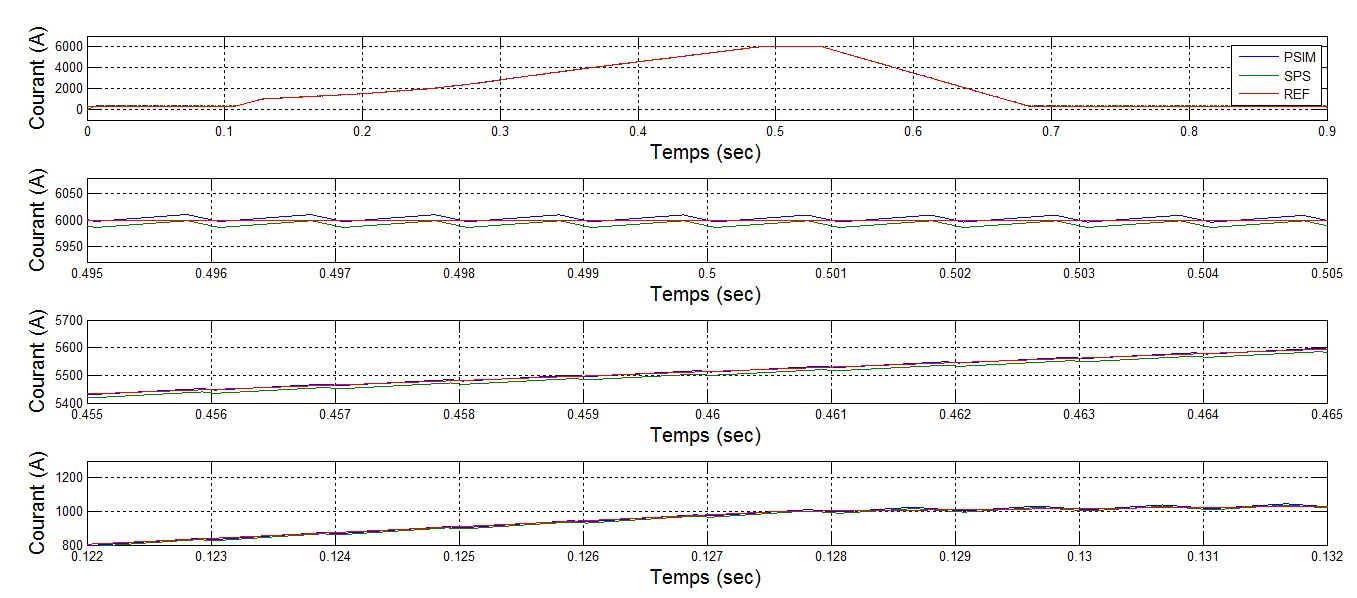
\includegraphics[scale=0.5]{Fig/Hach_AFE/50u/hach_cou_ch.jpg}
\caption{Le courant au niveau de la charge à 50$\mu$s}
\label{AF_HA_CHA50}
\end{figure}

\begin{figure}[htb]
\centering
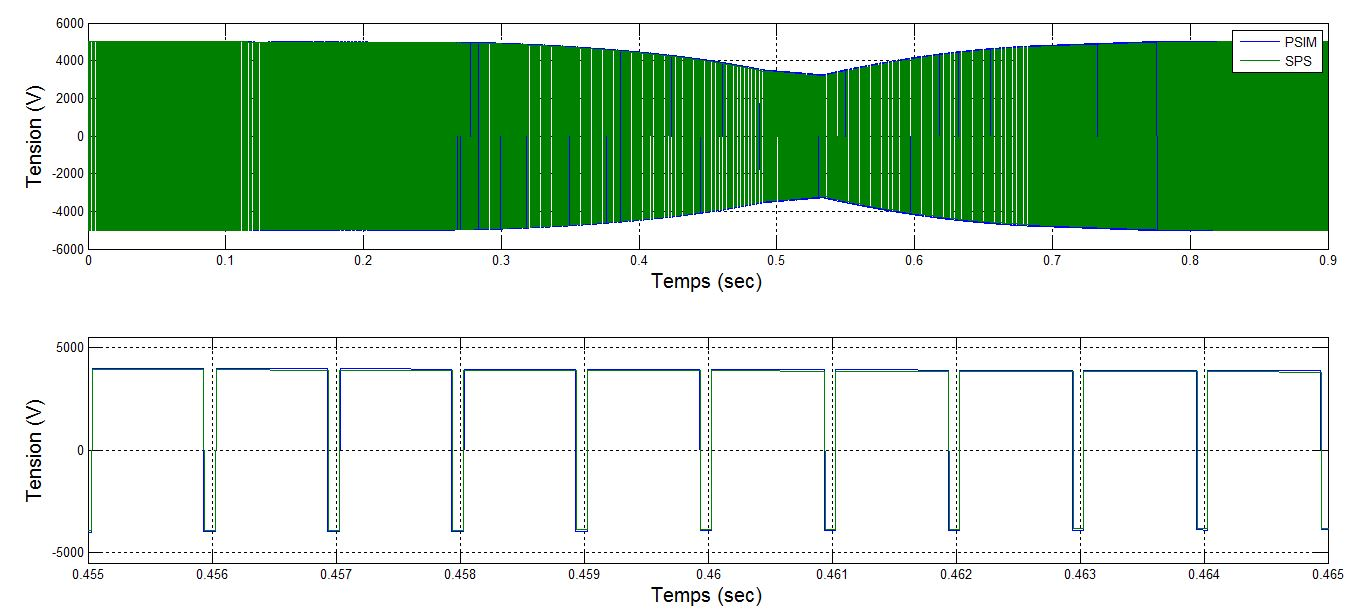
\includegraphics[scale=0.5]{Fig/Hach_AFE/50u/hach_ten_ch.jpg}
\caption{La tension au niveau de la charge à 50$\mu$s}
\label{AF_HA_CHV50}
\end{figure}

\begin{figure}[htb]
\centering
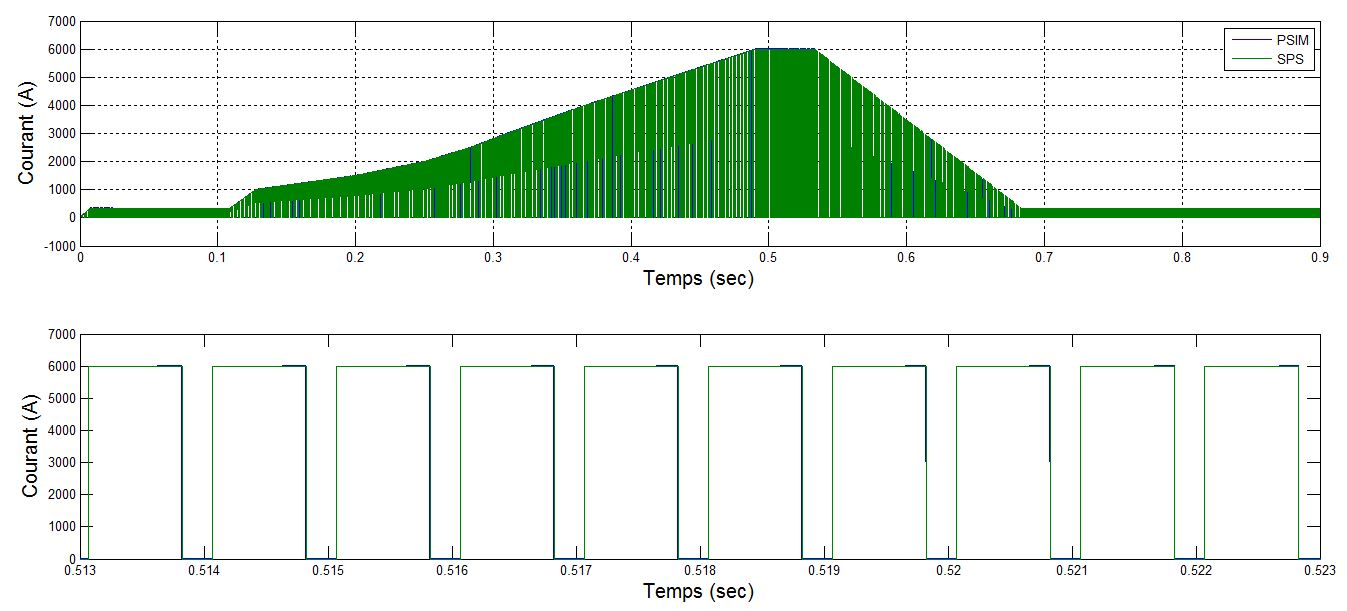
\includegraphics[scale=0.5]{Fig/Hach_AFE/50u/IGBT_cou_hach.jpg}
\caption{Le courant au niveau d'un IGBT à 50$\mu$s pour le hacheur 4 quadrants}
\label{AF_HA_HAA50}
\end{figure}

\begin{figure}[htb]
\centering
\includegraphics[scale=0.5]{Fig/Hach_AFE/50u/IGBT_ten_hach.jpg}
\caption{La tension au niveau d'un IGBT à 50$\mu$s pour le hacheur 4 quadrants}
\label{AF_HA_HAV50}
\end{figure}

\clearpage
\subsubsection{Vérification pour un pas de calcul de 5$\mu$s}

\begin{figure}[htb]
\centering
\includegraphics[scale=0.5]{Fig/Hach_AFE/5u/cour_al.jpg}
\caption{Le courant d'entrée à 5$\mu$s}
\label{AF_HA_cou5}
\end{figure}

\begin{figure}[htb]
\centering
\includegraphics[scale=0.5]{Fig/Hach_AFE/5u/ten_bus.jpg}
\caption{La tension au bus à 5$\mu$s}
\label{AF_HA_vc5h}
\end{figure}


\begin{figure}[htb]
\centering
\includegraphics[scale=0.5]{Fig/Hach_AFE/5u/IGBT_AFE.jpg}
\caption{La tension et le courant au niveau d'un IGBT à 5$\mu$s au niveau de l'AFE}
\label{AF_HA_IGBT5}
\end{figure}

\begin{figure}[htb]
\centering
\includegraphics[scale=0.5]{Fig/Hach_AFE/5u/hach_cou_ch.jpg}
\caption{Le courant au niveau de la charge à 5$\mu$s}
\label{AF_HA_CHA5}
\end{figure}

\begin{figure}[htb]
\centering
\includegraphics[scale=0.5]{Fig/Hach_AFE/5u/hach_ten_ch.jpg}
\caption{La tension au niveau de la charge à 5$\mu$s}
\label{AF_HA_CHV5}
\end{figure}

\begin{figure}[htb]
\centering
\includegraphics[scale=0.5]{Fig/Hach_AFE/5u/IGBT_cou_hach.jpg}
\caption{Le courant au niveau d'un IGBT à 5$\mu$s pour le hacheur 4 quadrants}
\label{AF_HA_HAA5}
\end{figure}

\begin{figure}[htb]
\centering
\includegraphics[scale=0.5]{Fig/Hach_AFE/5u/IGBT_ten_hach.jpg}
\caption{La tension au niveau d'un IGBT à 5$\mu$s pour le hacheur 4 quadrants}
\label{AF_HA_HAV5}
\end{figure}


\clearpage
\subsubsection{Vérification pour un pas de calcul de 1$\mu$s}

\begin{figure}[htb]
\centering
\includegraphics[scale=0.5]{Fig/Hach_AFE/1u/cour_al.jpg}
\caption{Le courant d'entrée à 1$\mu$s}
\label{AF_HA_cou1}
\end{figure}

\begin{figure}[htb]
\centering
\includegraphics[scale=0.5]{Fig/Hach_AFE/1u/ten_bus.jpg}
\caption{La tension au bus à 1$\mu$s}
\label{AF_HA_vch1}
\end{figure}


\begin{figure}[htb]
\centering
\includegraphics[scale=0.5]{Fig/Hach_AFE/1u/IGBT_AFE.jpg}
\caption{La tension et le courant au niveau d'un IGBT à 1$\mu$s au niveau de l'AFE}
\label{AF_HA_IGBT1}
\end{figure}

\begin{figure}[htb]
\centering
\includegraphics[scale=0.5]{Fig/Hach_AFE/1u/hach_cou_ch.jpg}
\caption{Le courant au niveau de la charge à 1$\mu$s}
\label{AF_HA_CHA1}
\end{figure}

\begin{figure}[htb]
\centering
\includegraphics[scale=0.5]{Fig/Hach_AFE/1u/hach_ten_ch.jpg}
\caption{La tension au niveau de la charge à 1$\mu$s}
\label{AF_HA_CHV1}
\end{figure}

\begin{figure}[htb]
\centering
\includegraphics[scale=0.5]{Fig/Hach_AFE/1u/IGBT_cou_hach.jpg}
\caption{Le courant au niveau d'un IGBT à 1$\mu$s pour le hacheur 4 quadrants}
\label{AF_HA_HAA1}
\end{figure}

\begin{figure}[htb]
\centering
\includegraphics[scale=0.5]{Fig/Hach_AFE/1u/IGBT_ten_hach.jpg}
\caption{La tension au niveau d'un IGBT à 1$\mu$s pour le hacheur 4 quadrants}
\label{AF_HA_HAV1}
\end{figure}


\subsection{AFE 3 level avec le DCP/DCN}
\subsubsection{Vérification pour un pas de calcul de 50$\mu$s}

\begin{figure}[htb]
\centering
\includegraphics[scale=0.5]{Fig/DCP_AFE/50u/cour_al.jpg}
\caption{Le courant d'entrée à 50$\mu$s}
\label{AF_DC_cou50}
\end{figure}

\begin{figure}[htb]
\centering
\includegraphics[scale=0.5]{Fig/DCP_AFE/50u/ten_bus.jpg}
\caption{La tension au bus à 50$\mu$s}
\label{AF_DC_vch50}
\end{figure}


\begin{figure}[htb]
\centering
\includegraphics[scale=0.5]{Fig/DCP_AFE/50u/IGBT_afe.jpg}
\caption{La tension et le courant au niveau d'un IGBT à 50$\mu$s au niveau de l'AFE}
\label{AF_DC_IGBT50}
\end{figure}

\begin{figure}[htb]
\centering
\includegraphics[scale=0.5]{Fig/DCP_AFE/50u/ten_diode_afe.jpg}
\caption{La tension et le courant au niveau d'une diode à 50$\mu$s au niveau de l'AFE}
\label{AF_DC_DI50}
\end{figure}



\begin{figure}[htb]
\centering
\includegraphics[scale=0.5]{Fig/DCP_AFE/50u/cour_ch.jpg}
\caption{Le courant au niveau de la charge à 50$\mu$s}
\label{AF_DC_CHA50}
\end{figure}

\begin{figure}[htb]
\centering
\includegraphics[scale=0.5]{Fig/DCP_AFE/50u/ten_ch.jpg}
\caption{La tension au niveau de la charge à 50$\mu$s}
\label{AF_DC_CHV50}
\end{figure}

\begin{figure}[htb]
\centering
\includegraphics[scale=0.5]{Fig/DCP_AFE/50u/hash_cou_IGBT.jpg}
\caption{Le courant au niveau d'un IGBT à 50$\mu$s pour le hacheur 4 quadrants}
\label{AF_DC_HAA50}
\end{figure}

\begin{figure}[htb]
\centering
\includegraphics[scale=0.5]{Fig/DCP_AFE/50u/hash_ten_IGBT.jpg}
\caption{La tension au niveau d'un IGBT à 50$\mu$s pour le hacheur 4 quadrants}
\label{AF_DC_HAV50}
\end{figure}


\begin{figure}[htb]
\centering
\includegraphics[scale=0.5]{Fig/DCP_AFE/50u/hash_diode_cou.jpg}
\caption{Le courant au niveau d'une diode à 50$\mu$s pour le hacheur 4 quadrants}
\label{AF_DC_HA50}
\end{figure}

\begin{figure}[htb]
\centering
\includegraphics[scale=0.5]{Fig/DCP_AFE/50u/hash_diode.jpg}
\caption{La tension au niveau d'une diode à 50$\mu$s pour le hacheur 4 quadrants}
\label{AF_DC_HV50}
\end{figure}

\clearpage
\subsubsection{Vérification pour un pas de calcul de 5$\mu$s}

\begin{figure}[htb]
\centering
\includegraphics[scale=0.5]{Fig/DCP_AFE/5u/cour_al.jpg}
\caption{Le courant d'entrée à 5$\mu$s}
\label{AF_DC_cou5}
\end{figure}

\begin{figure}[htb]
\centering
\includegraphics[scale=0.5]{Fig/DCP_AFE/5u/ten_bus.jpg}
\caption{La tension au bus à 5$\mu$s}
\label{AF_DC_vch5}
\end{figure}


\begin{figure}[htb]
\centering
\includegraphics[scale=0.5]{Fig/DCP_AFE/5u/IGBT_afe.jpg}
\caption{La tension et le courant au niveau d'un IGBT à 5$\mu$s au niveau de l'AFE}
\label{AF_DC_IGBT5}
\end{figure}

\begin{figure}[htb]
\centering
\includegraphics[scale=0.5]{Fig/DCP_AFE/5u/ten_diode_afe.jpg}
\caption{La tension et le courant au niveau d'une diode à 5$\mu$s au niveau de l'AFE}
\label{AF_DC_DI5}
\end{figure}



\begin{figure}[htb]
\centering
\includegraphics[scale=0.5]{Fig/DCP_AFE/5u/cour_ch.jpg}
\caption{Le courant au niveau de la charge à 5$\mu$s}
\label{AF_DC_CHA5}
\end{figure}

\begin{figure}[htb]
\centering
\includegraphics[scale=0.5]{Fig/DCP_AFE/5u/ten_ch.jpg}
\caption{La tension au niveau de la charge à 5$\mu$s}
\label{AF_DC_CHV5}
\end{figure}

\begin{figure}[htb]
\centering
\includegraphics[scale=0.5]{Fig/DCP_AFE/5u/hash_cou_IGBT.jpg}
\caption{Le courant au niveau d'un IGBT à 5$\mu$s pour le hacheur 4 quadrants}
\label{AF_DC_HAA5}
\end{figure}

\begin{figure}[htb]
\centering
\includegraphics[scale=0.5]{Fig/DCP_AFE/5u/hash_ten_IGBT.jpg}
\caption{La tension au niveau d'un IGBT à 5$\mu$s pour le hacheur 4 quadrants}
\label{AF_DC_HAV5}
\end{figure}


\begin{figure}[htb]
\centering
\includegraphics[scale=0.5]{Fig/DCP_AFE/5u/hash_diode_cou.jpg}
\caption{Le courant au niveau d'une diode à 5$\mu$s pour le hacheur 4 quadrants}
\label{AF_DC_HA5}
\end{figure}

\begin{figure}[htb]
\centering
\includegraphics[scale=0.5]{Fig/DCP_AFE/5u/hash_diode.jpg}
\caption{La tension au niveau d'une diode à 5$\mu$s pour le hacheur 4 quadrants}
\label{AF_DC_HV5}
\end{figure}


\clearpage
\subsubsection{Vérification pour un pas de calcul de 1$\mu$s}

\begin{figure}[htb]
\centering
\includegraphics[scale=0.5]{Fig/DCP_AFE/1u/cour_al.jpg}
\caption{Le courant d'entrée à 1$\mu$s}
\label{AF_DC_cou1}
\end{figure}

\begin{figure}[htb]
\centering
\includegraphics[scale=0.5]{Fig/DCP_AFE/1u/ten_bus.jpg}
\caption{La tension au bus à 1$\mu$s}
\label{AF_DC_vch1}
\end{figure}


\begin{figure}[htb]
\centering
\includegraphics[scale=0.5]{Fig/DCP_AFE/1u/IGBT_afe.jpg}
\caption{La tension et le courant au niveau d'un IGBT à 1$\mu$s au niveau de l'AFE}
\label{AF_DC_IGBT1}
\end{figure}

\begin{figure}[htb]
\centering
\includegraphics[scale=0.5]{Fig/DCP_AFE/1u/ten_diode_afe.jpg}
\caption{La tension et le courant au niveau d'une diode à 1$\mu$s au niveau de l'AFE}
\label{AF_DC_DI1}
\end{figure}



\begin{figure}[htb]
\centering
\includegraphics[scale=0.5]{Fig/DCP_AFE/1u/cour_ch.jpg}
\caption{Le courant au niveau de la charge à 1$\mu$s}
\label{AF_DC_CHA1}
\end{figure}

\begin{figure}[htb]
\centering
\includegraphics[scale=0.5]{Fig/DCP_AFE/1u/ten_ch.jpg}
\caption{La tension au niveau de la charge à 1$\mu$s}
\label{AF_DC_CHV1}
\end{figure}

\begin{figure}[htb]
\centering
\includegraphics[scale=0.5]{Fig/DCP_AFE/1u/hash_cou_IGBT.jpg}
\caption{Le courant au niveau d'un IGBT à 1$\mu$s pour le hacheur 4 quadrants}
\label{AF_DC_HAA1}
\end{figure}

\begin{figure}[htb]
\centering
\includegraphics[scale=0.5]{Fig/DCP_AFE/1u/hash_ten_IGBT.jpg}
\caption{La tension au niveau d'un IGBT à 1$\mu$s pour le hacheur 4 quadrants}
\label{AF_DC_HAV1}
\end{figure}


\begin{figure}[htb]
\centering
\includegraphics[scale=0.5]{Fig/DCP_AFE/1u/hash_diode_cou.jpg}
\caption{Le courant au niveau d'une diode à 1$\mu$s pour le hacheur 4 quadrants}
\label{AF_DC_HA1}
\end{figure}

\begin{figure}[htb]
\centering
\includegraphics[scale=0.5]{Fig/DCP_AFE/1u/hash_diode.jpg}
\caption{La tension au niveau d'une diode à 1$\mu$s pour le hacheur 4 quadrants}
\label{AF_DC_HV1}
\end{figure}


\end{document}